% ============================================================================
% main_v2.tex — PREVISUALIZACIÓN de la reescritura integral (v2)
% Estructura "STRATA como hilo" (6 capítulos) + abstract EN + anexo de demostraciones.
% No sustituye a main.tex hasta que Raquel apruebe la comparación v1 vs v2.
% Compilar:  latexmk -pdf -bibtex main_v2.tex
% ============================================================================
\documentclass[11pt,a4paper,oneside]{report}

% ============================================================================
% preamble.tex — paquetes, tipografía y comandos de la memoria del TFG (STRATA)
% Plantilla limpia propia (no hay plantilla UCM obligatoria salvo la portada).
% Documento A4 vertical, español. Citación NUMÉRICA con biblatex (backend biber).
% ============================================================================

% --- Idioma y codificación ---
\usepackage[utf8]{inputenc}
\usepackage[T1]{fontenc}
\usepackage[spanish,es-tabla]{babel}
\usepackage{csquotes}          % requerido por biblatex+babel para comillas correctas
\usepackage{microtype}
\frenchspacing

% --- Geometría A4 ---
\usepackage[a4paper,top=2.5cm,bottom=2.5cm,left=3cm,right=2.5cm]{geometry}
\usepackage{setspace}
\onehalfspacing

% --- Matemáticas ---
\usepackage{amsmath,amssymb,amsthm,mathtools}
\usepackage{bm}

\theoremstyle{plain}
\newtheorem{teorema}{Teorema}[chapter]
\newtheorem{proposicion}[teorema]{Proposición}
\newtheorem{lema}[teorema]{Lema}
\newtheorem{corolario}[teorema]{Corolario}
\theoremstyle{definition}
\newtheorem{definicion}[teorema]{Definición}
\newtheorem{ejemplo}[teorema]{Ejemplo}
\theoremstyle{remark}
\newtheorem{observacion}[teorema]{Observación}

% --- Figuras, tablas, código ---
\usepackage{graphicx}
\graphicspath{{figures/}}
\usepackage{booktabs}
\usepackage{multirow}
\usepackage{array}
\usepackage{float}
\usepackage{siunitx}
\usepackage{eurosym}

% --- Notación canónica del proyecto (coherente con glosario.md y el código) ---
\newcommand{\sigmat}{\sigma_t}                 % volatilidad condicional GARCH
\newcommand{\muk}{\mu_k}                        % media del régimen k
\newcommand{\rnext}{r_{t+1}}                    % retorno del día siguiente
\newcommand{\reglog}{r_t^{\log}}               % log-retorno
\newcommand{\gammaf}{\gamma^{f}_t}             % posterior filtrado del HMM
\newcommand{\RAM}{\mathrm{RAM}}
\newcommand{\PSA}{\mathrm{PSA}}
\newcommand{\GSO}{\mathrm{GSO}}
\newcommand{\E}{\mathbb{E}}
\newcommand{\Prob}{\mathbb{P}}
\newcommand{\Var}{\operatorname{Var}}
\newcommand{\sign}{\operatorname{signo}}
\newcommand{\indic}[1]{\mathbf{1}\{#1\}}

% --- Bibliografía: numérica en texto [n], lista numerada estilo APA-español ---
\usepackage[backend=biber,style=numeric,sorting=none,language=spanish]{biblatex}
\addbibresource{bibliography.bib}

% --- Hipervínculos (al final) ---
\usepackage[hidelinks]{hyperref}
\usepackage{cleveref}


\begin{document}

% --- Portada oficial UCM ---
% ============================================================================
% portada.tex — portada oficial UCM (réplica del modelo de la Facultad)
% ============================================================================
\begin{titlepage}
    \centering
    \vspace*{1cm}

    {\large\textbf{UNIVERSIDAD COMPLUTENSE DE MADRID}}\\[0.3cm]
    {\large\textbf{FACULTAD DE CIENCIAS MATEMÁTICAS}}

    \vspace{2.5cm}

    
\includegraphics[width=4.5cm]{figuras/logo_UCM}

    \vspace{2.5cm}

    {\large\textbf{TRABAJO DE FIN DE GRADO}}

    \vspace{4cm}

    {\large STRATA: supervisión estadística en tiempo real\\
    de un agente de trading basado en LLMs}

    \vspace{0.8cm}

    {\normalsize Tutor: Daniel Vélez Serrano}

    \vspace{3cm}

    {\Large\textbf{Raquel García Hernández}}

    \vspace{0.4cm}

    {\normalsize Doble Grado en Matemáticas y Ciencia de Datos}

    \vspace{0.4cm}

    {\normalsize Curso académico 2025-2026}

\end{titlepage}


% --- Resumen en inglés (normativa: pág. 3, 100-200 palabras) ---
\renewcommand{\abstractname}{Abstract}
\begin{abstract}
    Language-model agents already trade real money, and they are not deterministic: faced with the same question they answer differently, and they fail without warning. When capital is at stake, that is a problem. The agent studied here, a replica of AI Hedge Fund with five investor personalities over a single language model, decides a direction and a size for each asset every day. Left unsupervised it loses: on SPY it calls the next day's direction correctly only $36.6\%$ of the time, below a coin toss, and turns an initial \euro{}1000 into \euro{}700.

    STRATA answers that failure with supervision rather than replacement: an external statistical layer that audits every decision at runtime and overrides it when it contradicts an explicit model of the market. Three orthogonal classical detectors carry the audit—a hidden Markov regime model, a Bayesian online change-point detector and a GARCH volatility band. The whole design rests on a causal, out-of-sample protocol: the detectors are calibrated once, their thresholds closed before the evaluation begins, and every claim is settled by a paired test.

    The rescue is real, statistically significant and interpretable. The supervised decision beats the agent both in directional accuracy (paired McNemar) and in risk (an aggregated $\Delta$Sharpe whose $95\%$ interval excludes zero), and the effect runs through a single readable channel, the market regime. A free meta-learner, far from discarding the hand-built detectors, rediscovers them and ranks them above the agent's own signals. Across a panel of ten assets one property governs the result: the stronger an asset's leverage effect, the more supervision rescues it, with the regime rule leading on broad indices and the meta-learner on the rest. STRATA does not beat the market, and never set out to—its benchmark is the agent, not the market. Within that scope, classical statistics turn a systematically losing agent into one corrected in real time by a transparent, falsifiable rule.
    
    \medskip
    \noindent\textbf{Keywords:} runtime supervision, LLM trading agent, hidden Markov model, GARCH, change-point detection, meta-labeling, leverage effect.
    \end{abstract}
    

\tableofcontents
\cleardoublepage

% --- Capítulos (estructura v2: STRATA como hilo) ---
\chapter{Introducción}
\label{cap:introduccion}

\section{Problema. Motivación}
\label{sec:intro-motivacion}

Los agentes basados en grandes modelos de lenguaje ya toman decisiones de inversión. Con ese despliegue ha crecido una demanda concreta: supervisar de forma continua y trazable lo que la IA agéntica decide. A medida que estos sistemas ganan autonomía, sus decisiones se vuelven difíciles de seguir para un humano, y crece el interés en los \emph{guardrails}: una supervisión automática que acote lo que el agente puede hacer.

Muchas personas ya confían su dinero a inversiones gestionadas por estos agentes. Un agente LLM no es determinista: ante la misma pregunta puede responder de forma distinta, y no señala cuándo acierta o falla. En la gestión de capital, donde un solo error tiene coste elevado, esa indeterminación es crítica.

El sector financiero exige por ello un control más estricto. Los agentes LLM ejecutan las instrucciones con fidelidad antes que maximizar el beneficio \cite{lopezlira2025cantrade}, su confianza declarada está mal calibrada y son manipulables. Entre la supervisión que se reclama y una herramienta falsable que la ofrezca hay una distancia que este trabajo aborda.


El agente estudiado es una réplica de AI Hedge Fund: cinco personalidades inversoras sobre un mismo modelo de lenguaje que deciden, para cada activo y cada día, una dirección y un tamaño. Sin supervisión pierde dinero. Sobre SPY acierta la dirección el $0{,}366$ de los días, por debajo de lo que daría una moneda, y una inversión inicial de \euro{}1000 termina en \euro{}700.\,% fuente: cap. STRATA-SPY (SPY M5: acc 0,366, equity 0,70)
El fenómeno no es propio de SPY: el agente acierta por debajo del medio punto en siete de los diez activos del panel.\,% fuente: cap. panel (7/10 < 0,5)

La pérdida tiene estructura. El agente mantiene una posición casi rígida que apenas atiende a la señal del día. Un fallo sistemático se puede corregir desde fuera; ese es el problema que aborda este trabajo.

\section{Propuesta: supervisión estadística externa}
\label{sec:intro-idea}

STRATA es la solución a este problema: un supervisor estadístico exógeno que audita cada decisión en tiempo de ejecución y la rectifica cuando contradice el comportamiento del mercado. Se apoya en tres detectores ortogonales, cada uno sobre un modelo estadístico clásico que el capítulo~\ref{cap:strata} formaliza: RAM mira la coherencia de la apuesta con el régimen de mercado, PSA la coherencia temporal de las decisiones del agente y GSO la compatibilidad del tamaño con la volatilidad. Cuando uno se dispara, STRATA actúa sobre la decisión: la registra, atenúa su tamaño o la sustituye. La corrección se contrasta de forma pareada contra el mismo agente sin supervisar, decisión a decisión.

La idea de una etapa secundaria que vigila a un modelo primario no es nueva: el \emph{meta-labeling} de López de Prado \cite{lopezdeprado2018} añade un segundo modelo que decide si actuar sobre la señal del primero. STRATA recoge esa lógica y la lleva más lejos. Aquí el primario es el agente LLM, y el supervisor son tres detectores estadísticos clásicos que juzgan su decisión desde ejes independientes y la registran, atenúan o sustituyen. La intervención es exógena: depende de lo que los detectores leen del mercado, no de lo que el agente declare. Eso la separa del equipo de riesgo de TradingAgents \cite{xiao2024tradingagents}, un agente deliberativo interno que comparte la información y los sesgos del sistema.

\chapter{Objetivos}
\label{cap:objetivos}

El capítulo anterior dejó el problema sobre la mesa: un agente LLM que decide con dinero real pierde la dirección y el capital, y lo hace de forma sistemática. Este capítulo fija qué se propone el trabajo frente a ese problema, la hipótesis que pone a prueba y cómo la contrasta.

\section{Hipótesis}
\label{sec:obj-hipotesis}

La pregunta de investigación es si una capa de supervisión estadística externa puede rescatar a un agente LLM cuando pierde. La formulamos como una afirmación que puede refutarse:

\begin{quote}
Filtrar o atenuar las decisiones de un agente LLM de trading con detectores estadísticos clásicos rescata al agente de forma significativa cuando este pierde dinero y acierta la dirección menos de la mitad de las veces.
\end{quote}

La hipótesis nula es que la supervisión no cambia nada: las decisiones supervisadas no se distinguen de las del agente solo, ni en acierto direccional ni en riesgo. Para poder rechazarla fijamos de antemano el contraste de cada nivel y un criterio de fracaso, de modo que un resultado contrario refute la hipótesis en lugar de maquillarla.

\section{Objetivo general}
\label{sec:obj-general}

Demostrar, con rigor estadístico, que supervisar en tiempo de ejecución las decisiones de un agente LLM de trading con detectores estadísticos clásicos rescata al agente cuando pierde, y caracterizar cuándo y por qué funciona. No se persigue batir al mercado ni generar alfa: el alcance es la supervisión, y el listón es el propio agente, no una referencia pasiva.

\section{Objetivos específicos}
\label{sec:obj-especificos}

\begin{enumerate}
  \item Formalizar tres detectores estadísticos clásicos (régimen con un HMM, cambio estructural con BOCPD y volatilidad con GARCH) que auditen cada decisión del agente en tiempo de ejecución, junto con el protocolo de medición causal y sin fuga que los evalúa (capítulo~\ref{cap:strata}).
  \item Probar, con contrastes pareados, si esa supervisión rescata al agente cuando pierde, tanto en acierto direccional (McNemar y \emph{sign test}) como en riesgo ($\Delta$Sharpe con \emph{bootstrap}), primero sobre el caso de SPY y luego sobre el panel (capítulos~\ref{cap:spy} y~\ref{cap:panel}).
  \item Atribuir el efecto a cada detector y caracterizar en qué activos funciona la supervisión y por qué, a través de la anatomía de la intervención, la compuerta de régimen y el patrón que liga la naturaleza del activo con el canal que lo rescata (capítulos~\ref{cap:spy} y~\ref{cap:panel}).
  \item Comprobar si un meta-learner libre redescubre las señales de STRATA en lugar de prescindir de ellas, contrastando atribución (valores de Shapley y ablación) y equivalencia frente a la regla (capítulo~\ref{cap:panel}).
  \item Delimitar el alcance honesto de la técnica: declarar dónde no aporta (frente a una referencia trivial y en activos de apalancamiento débil), con el mismo rigor con que se reporta lo que sí aporta (capítulo~\ref{cap:panel}).
\end{enumerate}

\section{Plan de trabajo}
\label{sec:obj-plan}

La memoria sigue este orden. El capítulo~\ref{cap:estado-arte} sitúa el trabajo entre los agentes LLM de trading, la supervisión en tiempo de ejecución y los modelos clásicos de régimen y volatilidad. El capítulo~\ref{cap:strata} formaliza los tres detectores, las estrategias que derivan de ellos y el protocolo de medición fuera de muestra. El capítulo~\ref{cap:spy} lleva STRATA al caso de SPY, paso a paso. El capítulo~\ref{cap:panel} prueba el rescate sobre el panel de diez activos y busca el patrón que lo ordena. Cierran las conclusiones y el trabajo futuro (capítulo~\ref{cap:conclusiones}).

\chapter{Estado del arte}
\label{cap:estado-arte}

Nuestro problema a tratar vive en el cruce de tres líneas que han avanzado por separado: los agentes LLM que ya operan en los mercados, la idea de supervisar un sistema mientras decide, y los modelos clásicos que describen el régimen de mercado y su riesgo. Recorremos las tres y dejamos ver el hueco que STRATA ocupa.

\section{Agentes LLM en finanzas}
\label{sec:agentes-llm}

Un gran modelo de lenguaje (LLM) es una red que predice la siguiente palabra a partir del contexto, mediante un mecanismo de atención \cite{vaswani2017attention}. Por sí solo solo escribe: se vuelve un \emph{agente} cuando lo envolvemos en un bucle que razona, llama a herramientas y actúa sobre un entorno \cite{yao2023react, wang2024survey}. De ahí salieron sistemas que deciden inversiones en lugar de redactar \cite{yang2023fingpt}. El foco se desplazó pronto de si un modelo entiende los mercados a cómo coordinar varios, y hoy domina la arquitectura multiagente: varias personalidades inversoras deliberan y un gestor modera la posición final \cite{xiao2024tradingagents, zhao2025alphaagents}. El control de riesgo que incorporan vive dentro del propio sistema y comparte sus sesgos: el equipo de riesgo de TradingAgents razona en lenguaje natural \cite{xiao2024tradingagents} y AlphaAgents ajusta la cartera a la tolerancia del inversor \cite{zhao2025alphaagents}, pero ninguno audita con un modelo estadístico externo si cada decisión es coherente con el mercado observado.

 Los agentes LLM ejecutan las instrucciones con fidelidad antes que maximizar beneficio, aun cuando eso les hace perder \cite{lopezlira2025cantrade}, y su confianza declarada está peor calibrada que la de un humano: se muestran sobreconfiados justo cuando fallan \cite{sung2025grace, damani2025rlcr}. Cambian de estilo inversor sin que el cambio responda a su propio criterio \cite{li2026behavioral} y resultan manipulables ante datos diseñados para engañarlos \cite{yan2025tradetrap}. Un agente rígido cuya certeza no es fiable pide un supervisor exógeno. Y la evaluación es frágil: muchos resultados optimistas no aguantan una validación temporal honesta \cite{li2025deepfund}, y el \emph{look-ahead} infla las métricas cuando el periodo de prueba cae dentro del preentrenamiento \cite{benhenda2026lookahead}; por eso nuestra ventana fuera de muestra empieza tras el corte de entrenamiento del modelo.

El agente que estudiamos es una réplica de AI Hedge Fund \cite{singh2024aihedgefund}, un sistema de cinco personalidades que emulan a inversores reconocidos (Buffett, Wood, Druckenmiller, Burry y Ackman) sobre un mismo modelo de lenguaje. Para cada activo y día cada personalidad emite una señal direccional con un grado de confianza; un agente de riesgo fija el límite de posición según la volatilidad, y un gestor integra las cinco señales y ese límite en una sola decisión, dirección y tamaño, por criterio propio y no por voto. Esa decisión diaria es lo que STRATA supervisa. Sin supervisión el agente reproduce los problemas anteriores: pierde dirección y dinero sobre SPY y la mayoría del panel (Sección~\ref{sec:intro-motivacion}). Lo llamamos M5, y la estructura de su pérdida importa más que el tamaño: mantiene una posición casi constante que apenas atiende a la señal del día. Un fallo sistemático se corrige desde fuera, y ahí entra una capa que reintroduzca esa información.

\section{Supervisión en tiempo de ejecución}
\label{sec:supervision}

La industria ya pide vigilar a estos agentes mientras operan. El discurso profesional lo resume en una consigna, \emph{guardrails, but no handcuffs}: barreras que acoten al agente sin maniatarlo, con monitorización continua, trazas de auditoría y salidas que escalen a un humano \cite{milligan2024guardrails}. Entre los controles aparece, casi de pasada, la \emph{validación estadística}: que las salidas se alineen con normas estadísticas realistas \cite{milligan2024guardrails}. La demanda queda en eslogan, sin decir qué norma, qué contraste ni cómo se mide que la corrección funcione. STRATA lo convierte en detectores falsables con contraste pareado.

Vigilar mientras se decide enlaza con la detección de anomalías \cite{chandola2009anomaly} y con el control en tiempo de ejecución (\emph{runtime enforcement}), que intercepta cada acción y bloquea la que incumple una condición \cite{wang2025agentspec, flehmig2025reliability}. Una regla declarativa codifica qué está prohibido; nosotros modelamos cómo de coherente es una posición con el estado del mercado, con tres detectores estadísticos clásicos e interpretables: RAM mira la coherencia con el régimen (modelo de Markov oculto), PSA la coherencia temporal del agente (puntos de cambio bayesianos) y GSO la compatibilidad del tamaño con la volatilidad (GARCH). Los tres descansan en cómo se describe hoy el régimen de mercado y su riesgo.

\section{Régimen de mercado y riesgo}
\label{sec:regimen}

La idea de fondo de RAM viene de Hamilton: una serie financiera no responde a un único mecanismo, sino que atraviesa estados latentes con propiedades estadísticas distintas y cambia de estado sin que lo veamos, de modo que la distribución de cada retorno depende del estado vigente \cite{hamilton1989}. Condicionar la cartera al régimen mejora las decisiones de forma apreciable \cite{ang2002regime, guidolin2007regime}. Sobre el eje continuo de la volatilidad opera la idea que ancla a GSO: dimensionar la posición para alcanzar una volatilidad objetivo (el \emph{volatility targeting}) mejora las propiedades de la serie de retornos \cite{moreira2017}. La literatura usa de dos \cite{ang2002regime} a cuatro \cite{guidolin2007regime} estados; usamos tres (calma, estrés y crisis): la verosimilitud fuera de muestra descarta dos y por encima de tres se pierde lectura. El régimen funciona como proxy direccional solo de forma condicional, y esa condición sostiene y limita la tesis: el \emph{leverage effect} de los índices agregados hace que en activos como SPY los estados de alta volatilidad coincidan con tramos bajistas, de modo que conocer el régimen informa del signo probable del retorno \cite{black1976, christie1982}. El régimen no predice el retorno: ordena las decisiones del agente. La coincidencia se diluye en valores con apalancamiento débil, donde el régimen pierde poder direccional, y ahí está el límite de la técnica. Estas tres líneas se han tocado por separado; STRATA las une con detectores estadísticos clásicos y exógenos, que el capítulo siguiente formaliza.

\chapter{Fundamentos teóricos y diseño de STRATA}
\label{cap:strata}

Las tres líneas del capítulo anterior —agentes LLM de trading, supervisión en tiempo de ejecución y modelos clásicos de régimen y volatilidad— no se habían combinado sobre un mismo agente. STRATA aborda esa combinación. Este capítulo reúne la base matemática que la sostiene y fija la notación del resto de la memoria: los tres detectores y la capa que convierte sus señales en intervención, las estrategias que aprenden sobre esas señales y el protocolo de medición del rescate. El caso de SPY, donde el sistema se pone a prueba, queda para el capítulo~\ref{cap:spy}.

\section{Los detectores: RAM, PSA y GSO}
\label{sec:strata-detectores}

\subsection{Preliminares y notación}
\label{sec:preliminares}

El punto de partida es una serie de precios diarios de un activo. Sea $P_t > 0$ el precio de cierre del día $t$, con $t \in \{0, 1, \dots, T\}$. La cantidad relevante no es el precio en sí, sino su variación relativa de un día al siguiente, el \emph{log-retorno}
\[
\reglog \;=\; \log\!\left(\frac{P_t}{P_{t-1}}\right) \;=\; \log P_t - \log P_{t-1}, \qquad t \ge 1,
\]
El log-retorno mide el crecimiento del precio en escala logarítmica; es positivo cuando el precio sube y negativo cuando baja.

El \emph{retorno simple} $R_t = (P_t - P_{t-1})/P_{t-1}$, la fracción ganada o perdida, se relaciona con él por $\reglog = \log(1 + R_t)$. La ventaja del log-retorno es su aditividad temporal: el retorno acumulado entre los días $t_0$ y $t_0 + n$, en escala logarítmica, es la suma de los log-retornos diarios,
\[
\log\!\left(\frac{P_{t_0+n}}{P_{t_0}}\right)
= \log\!\left(\prod_{j=1}^{n} \frac{P_{t_0+j}}{P_{t_0+j-1}}\right)
= \sum_{j=1}^{n} \log\!\left(\frac{P_{t_0+j}}{P_{t_0+j-1}}\right)
= \sum_{j=1}^{n} r^{\log}_{t_0+j}.
\]
El retorno simple, en cambio, se compone de forma multiplicativa, $1 + R_{[t_0, t_0+n]} = \prod_{j=1}^{n}(1 + R_{t_0+j})$, lo que complica cualquier análisis que sume o promedie a lo largo del tiempo. Esa aditividad justifica modelar $\reglog$ en lo que sigue.

Se fija también la convención temporal que gobierna toda la validación y todo el backtest. La decisión de cartera tomada con la información disponible hasta el día $t$ no puede recompensarse con el movimiento de ese mismo día, que ya ha ocurrido. Por eso, para evitar el \emph{look-ahead}, el retorno que se contabiliza frente a una posición tomada en $t$ es el del día siguiente,
\[
\rnext \;=\; \log\!\left(\frac{P_{t+1}}{P_t}\right).
\]
Así se asegura la ausencia de fuga temporal: en adelante, todo producto entre una posición y un retorno usa $\rnext$.


Por último, una medida de cuánto se mueve el activo en un tramo de tiempo. Dada una ventana de $h$ días que termina en $t$, se define la \emph{volatilidad realizada}
\[
RV_t \;=\; \sqrt{\sum_{j=0}^{h-1} \big(r^{\log}_{t-j}\big)^2}\,,
\]
esto es, la raíz de la suma de cuadrados de los log-retornos de la ventana. $RV_t$ es un estimador no paramétrico de la dispersión local de los retornos: crece cuando el activo encadena días de movimientos grandes y se reduce en los tramos planos. A diferencia de la volatilidad condicional $\sigmat$ que se introduce en la Sección~\ref{sec:garch}, $RV_t$ no presupone ningún modelo; es una lectura directa de los datos.

Las series de retornos financieros no se comportan como ruido blanco gaussiano. Tres regularidades empíricas, documentadas de forma sistemática en la literatura \cite{cont2001}, motivan los modelos del resto del capítulo. La primera es que la distribución de los retornos tiene \emph{colas pesadas}: los movimientos extremos son mucho más frecuentes de lo que predice una normal, lo que lleva a sustituir la gaussiana por una distribución de colas anchas como la $t$ de Student en el modelo de volatilidad. El \emph{agrupamiento de volatilidad} es la segunda: los días de gran movimiento tienden a seguirse unos a otros, así que la magnitud de los retornos sí está correlada en el tiempo aunque su signo apenas lo esté, y eso es lo que captura un modelo GARCH. Queda la tercera, la \emph{poca autocorrelación} de los retornos en niveles: casi nula a partir del primer rezago, mientras que sus cuadrados o sus valores absolutos sí la presentan. La combinación de las tres sugiere que el comportamiento del activo alterna entre estados o regímenes con dinámicas distintas, idea que el modelo de cambio de régimen formaliza.

\subsection{La salida del agente}
\label{sec:agente-salida}

El objeto que STRATA supervisa es la decisión diaria de un agente de trading construido sobre un modelo de lenguaje. Las cinco personalidades y la arquitectura multiagente del fondo se describieron en la Sección~\ref{sec:agentes-llm}. Para la capa de supervisión, lo que importa es la salida: cada día, y para cada activo, el agente emite una dirección, un tamaño y la confianza con que los emite. La Sección~\ref{sec:strata-tecnico} la formaliza como una posición $w_t \in [-1, +1]$, el objeto sobre el que actúan los detectores. Las señales de las cinco personalidades reaparecen además como variables de entrada del meta-learner de la Sección~\ref{sec:sup-problema}, junto a las lecturas estadísticas de STRATA.

STRATA trata al agente como una caja negra: supervisa su decisión sin abrir el modelo ni reconstruir su razonamiento. Es la respuesta natural a sus dos rasgos. El modelo es opaco, su salida no tiene forma cerrada y su entrenamiento pudo ver parte del periodo de prueba; frente a eso, una capa externa que contrasta la decisión con un modelo explícito del mercado es más fiable que confiar en la coherencia interna del propio agente. El capítulo~\ref{cap:spy} documenta que esa decisión, sobre el caso de estudio, acierta la dirección menos de la mitad de los días, con un fallo sistemático y por tanto corregible desde fuera.

\subsection{STRATA a nivel técnico}
\label{sec:strata-tecnico}

Cada día, el agente de trading toma una decisión sobre el activo, resumida en una terna: un \emph{signo} (comprar o vender), un \emph{tamaño} y una \emph{confianza}. Esa terna determina una \emph{posición} $w_t \in [-1, +1]$, donde el signo marca la dirección (larga si $w_t > 0$, corta si $w_t < 0$) y el módulo $|w_t|$ es la fracción de capital expuesta; la posición tomada en $t$ se evalúa contra el retorno del día siguiente, $w_t \cdot \rnext$. STRATA no decide por el agente: \emph{supervisa} esa decisión. Formalmente, con $\mathcal{A}$ el espacio de decisiones del agente y $\mathcal{M}_t$ la información de mercado disponible hasta el día $t$ (resumida en $x_{1:t}$), STRATA es la aplicación
\[
\mathrm{STRATA}\colon \mathcal{A} \times \mathcal{M}_t \longrightarrow [0,1]^3,
\qquad
(w_t,\, x_{1:t}) \longmapsto \big(\mathrm{RAM}_t,\, \mathrm{PSA}_t,\, \mathrm{GSO}_t\big),
\]
que a partir de la decisión del agente y de una lectura estadística del mercado produce tres \emph{señales} sobre esa decisión, cada una en $[0,1]$. STRATA no predice el retorno: mide en qué grado la decisión del agente es coherente con el estado del mercado.

Las señales provienen de tres detectores, cada uno a cargo de un eje distinto. \textbf{RAM} se centra en el régimen: comprueba si la dirección de la apuesta encaja con el estado de mercado que el modelo oculto de Markov de la Sección~\ref{sec:hmm} considera vigente. \textbf{PSA} atiende al propio agente; con la detección bayesiana de puntos de cambio vigila si éste cambia de criterio de forma estructural, no por una simple fluctuación. \textbf{GSO} se ocupa del tamaño de la apuesta: contrasta el módulo de la posición con la volatilidad que estima el GARCH de la Sección~\ref{sec:garch}, y salta cuando la apuesta es grande para la volatilidad del mercado. Esta ortogonalidad de las tres dimensiones permite que cada detector capte algo que los otros dos no.

La intervención puede ir desde solo registrar la señal hasta reducir la posición o sustituirla por completo. Solo se analiza la variante más fuerte, que reorienta el signo de $w_t$ hacia el régimen cuando la incoherencia es alta; los modos intermedios quedan como trabajo futuro. La Sección~\ref{sec:strata-aplicado} detalla cómo se construye cada señal a partir de su detector y cuándo actúa esta intervención.

Conviene distinguir desde el principio entre la capa de señales y las reglas que las consumen. STRATA designa siempre la capa que produce las señales; M8 y M10 son estrategias que la utilizan. \textbf{M8} es una regla determinista de umbrales fijos, la capa de intervención que se detalla en la Sección~\ref{sec:strata-intervencion}, y sirve de referencia interpretable. \textbf{M10}, en cambio, no aplica umbrales fijos: es un modelo de segundo nivel (un \emph{meta-learner}) que toma como entradas las salidas del agente y de los detectores de STRATA y aprende a combinar esas señales para decidir la dirección del día siguiente. Se entrena solo con el pasado y es el objeto central del caso de estudio, que se desarrolla en el capítulo~\ref{cap:spy}.

\subsection{Modelos de cambio de régimen: HMM gaussiano}
\label{sec:hmm}

RAM necesita una lectura del estado de mercado. Esa lectura nace de la idea de que el mercado no se comporta siempre igual, sino que atraviesa fases distintas —calma, estrés, crisis— que no se observan pero se infieren de los retornos. Hamilton formalizó esta idea para series económicas mediante un proceso de Markov sobre estados no observados \cite{hamilton1989}: el régimen sigue una cadena de Markov y, condicionado a él, la serie observada se distribuye según los parámetros de ese régimen. Los tres regímenes se interpretan como \emph{Calma} (media ligeramente positiva, volatilidad baja), \emph{Estrés} (intermedio) y \emph{Crisis} (volatilidad alta, media negativa).

\subsubsection{Definición del HMM gaussiano}
\label{sec:hmm-def}

Un \emph{modelo oculto de Markov} (HMM) consta de una cadena de estados ocultos y una secuencia de observaciones que esos estados generan \cite{rabiner1989, cappe2005}. Sea $z_t \in \{1, \dots, K\}$ el estado oculto (el régimen) en el día $t$. La sucesión $\{z_t\}$ es una cadena de Markov homogénea de primer orden, con \emph{matriz de transición} $A_{ij} = \Prob(z_{t+1} = j \mid z_t = i)$ ($A_{ij}\ge 0$, $\sum_j A_{ij}=1$) y \emph{distribución inicial} $\pi_k = \Prob(z_1 = k)$. El estado no se observa; lo observado es $x_t$, el vector de características del día $t$ (el log-retorno y la volatilidad realizada $\mathrm{RV}_t$ con ventana de $21$ días). Suponemos \emph{emisiones gaussianas},
\[
x_t \mid z_t = k \;\sim\; \mathcal{N}(\muk, \Sigma_k),
\qquad b_k(x) = \mathcal{N}(x \mid \muk, \Sigma_k),
\]
y dos hipótesis de independencia condicional, palanca de toda derivación posterior: la observación de cada día depende solo del estado de ese día,
\[
\Prob(x_t \mid z_t, z_{t-1}, \dots, z_1, x_{t-1}, \dots, x_1) = \Prob(x_t \mid z_t) = b_{z_t}(x_t),
\tag{$\ast$}
\]
y la dinámica de los estados es markoviana de primer orden. El conjunto de parámetros es $\lambda = (A, \pi, \{\muk, \Sigma_k\}_{k=1}^{K})$, y la verosimilitud observada marginaliza sobre las trayectorias ocultas, $\Prob(x_{1:T} \mid \lambda) = \sum_{z_{1:T}} \Prob(x_{1:T}, z_{1:T} \mid \lambda)$. Esta suma recorre $K^T$ trayectorias; el algoritmo \emph{forward} la calcula en tiempo lineal en $T$.

\subsubsection{Algoritmo forward y filtrado causal}
\label{sec:hmm-forward}
\label{sec:hmm-filtrado}

La \emph{variable forward} $\alpha_t(k) = \Prob(x_{1:t},\, z_t = k \mid \lambda)$ recupera la verosimilitud completa por marginalización, $\Prob(x_{1:T} \mid \lambda) = \sum_{k} \alpha_T(k)$, y admite una recursión que evita la suma exponencial \cite{rabiner1989, bishop2006}.

\begin{proposicion}[Recursión forward]
\label{prop:forward}
Para $t \ge 1$ se tiene la inicialización $\alpha_1(k) = \pi_k\, b_k(x_1)$ y, para todo $j \in \{1, \dots, K\}$,
\[
\alpha_{t+1}(j) \;=\; b_j(x_{t+1}) \sum_{k=1}^{K} \alpha_t(k)\, A_{kj}.
\]
\end{proposicion}

La demostración está en el Anexo~\ref{anx:forward}. La recursión reduce el coste de $K^T$ a $\mathcal{O}(T K^2)$; en la práctica se trabaja en escala logarítmica para evitar el desbordamiento numérico.

Para decidir interesa la probabilidad del régimen \emph{dado} lo observado, el \emph{posterior filtrado} $\gammaf(k) = \Prob(z_t = k \mid x_{1:t})$, que se obtiene normalizando la variable forward \cite{rabiner1989, bishop2006}.

\begin{proposicion}[Filtrado a partir del forward]
\label{prop:filtrado}
Para todo $t \ge 1$ y todo $k$,
\[
\gammaf(k) \;=\; \frac{\alpha_t(k)}{\sum_{j=1}^{K} \alpha_t(j)}.
\]
\end{proposicion}

\begin{corolario}[Causalidad del filtrado]
\label{cor:causal}
Para cada $t$, el posterior filtrado $\gammaf$ es función únicamente de las observaciones $x_{1:t}$. En particular, puede calcularse en tiempo real el día $t$ sin recurrir a ninguna observación posterior.
\end{corolario}

La demostración de ambos está en el Anexo~\ref{anx:filtrado}. Esa causalidad es lo que permite usar el filtrado en producción. Contrasta con el \emph{posterior suavizado} $\Prob(z_t = k \mid x_{1:T})$, que condiciona sobre la secuencia completa y se calcula con el algoritmo forward-backward \cite{baum1970, rabiner1989}: estima mejor el régimen pasado porque incorpora lo ocurrido después, pero por eso mismo introduciría \emph{look-ahead} en una decisión. Por tanto \textbf{STRATA usa exclusivamente el posterior filtrado $\gammaf$}, nunca el suavizado: solo así, por el Corolario~\ref{cor:causal}, el sistema es reproducible en tiempo real.

\subsubsection{Estimación, trayectoria óptima y número de estados}
\label{sec:hmm-em}
\label{sec:hmm-viterbi}
\label{sec:hmm-K}

Los parámetros $\lambda$ se estiman por el algoritmo de Baum-Welch, instancia del esquema esperanza-maximización (EM) \cite{baum1970, dempster1977}. El paso E calcula los posteriores suavizados de estados y transiciones con el forward-backward —legítimo aquí, porque el ajuste se hace una sola vez fuera de línea sobre la calibración, no en una decisión en tiempo real—, y el paso M reestima los parámetros con fórmulas cerradas (Anexo~\ref{anx:em-pasos}): la distribución inicial y la matriz de transición como frecuencias esperadas, las medias y covarianzas como promedios ponderados por el posterior del estado.

\begin{lema}[Monotonía de EM]
\label{lem:em}
Sea $\lambda'$ el conjunto de parámetros que produce un paso de EM a partir de $\lambda$. Entonces la verosimilitud observada no decrece, $\Prob(x_{1:T} \mid \lambda') \ge \Prob(x_{1:T} \mid \lambda)$.
\end{lema}

La demostración está en el Anexo~\ref{anx:em}. El óptimo alcanzado es local y depende de la inicialización, de ahí la importancia de fijar la semilla. Una pregunta distinta al filtrado puntual es la \emph{trayectoria} de estados más probable, $z_{1:T}^{\ast} = \arg\max_{z_{1:T}} \Prob(z_{1:T} \mid x_{1:T}, \lambda)$, que resuelve el algoritmo de Viterbi por programación dinámica, con una recursión análoga a la del forward que sustituye la suma por un máximo \cite{viterbi1967} (Anexo~\ref{anx:viterbi}). Encadenar los modos del filtrado, $\arg\max_k \gammaf(k)$, no da en general la misma secuencia que Viterbi, que respeta las transiciones de $A$. El detector de régimen se apoya en el filtrado puntual por la exigencia de causalidad; Viterbi se usa de forma auxiliar para la lectura interpretativa sobre la calibración. El número de estados se fija combinando la log-verosimilitud held-out sobre un tramo de validación posterior en el tiempo \cite{rabiner1989} con la exigencia de interpretabilidad económica; ambos criterios fijan $K = 3$ como calibración de referencia, con los estados calma, estrés y crisis. Esta decisión se desarrolla en el capítulo siguiente.

\subsection{Volatilidad condicional: ARCH y GARCH(1,1)-t}
\label{sec:garch}

GSO se ocupa del tamaño de la apuesta, y para juzgarlo necesita una medida de cuánto se mueve el mercado ahora mismo. El HMM reparte la volatilidad en unos pocos estados discretos, una lectura útil pero gruesa: dentro de un mismo régimen, la dispersión de los retornos sube y baja de forma continua. El modelo GARCH captura justamente esa volatilidad que cambia día a día, y es el que alimenta a GSO.

\subsubsection{Heterocedasticidad condicional y modelo GARCH$(1,1)$-$t$}
\label{sec:garch-intro}
\label{sec:garch-arch}
\label{sec:garch-t}

Una serie de retornos es una realización de un proceso estocástico cuya ley conjunta factoriza en distribuciones condicionales sobre la filtración $\mathcal{F}_{t-1}$ \cite{hamilton1994, tsay2010}. Las regularidades empíricas de la Sección~\ref{sec:preliminares} muestran que el signo de los retornos es casi impredecible mientras su magnitud se agrupa en el tiempo: la varianza condicional depende del pasado. Esta \emph{heterocedasticidad condicional} —la diferencia entre incorrelación e independencia— es lo que los modelos ARCH explotan \cite{cont2001}. El retorno se modela como $\reglog = \mu + \epsilon_t$ con innovación $\epsilon_t = \sigmat\, \eta_t$, $\eta_t$ i.i.d. de media $0$ y varianza $1$; $\mu$ se toma constante porque en niveles los retornos son incorrelados, y toda la dinámica queda en $\sigmat^2 = \Var(\epsilon_t \mid \mathcal{F}_{t-1})$. Se distinguen dos nociones de estacionariedad: la \emph{estacionariedad en covarianza}, que exige media y autocovarianzas invariantes en el tiempo, y la \emph{estricta}, invariancia de la ley conjunta de cualquier bloque frente a traslación \cite{brockwell1991}.

Engle introdujo el \emph{ARCH} haciendo la varianza función de los errores recientes al cuadrado \cite{engle1982}, pero reproducir la persistencia observada exigía orden alto y muchos parámetros. Bollerslev lo generalizó al \emph{GARCH}, que añade la propia varianza pasada y logra la persistencia con pocos parámetros \cite{bollerslev1986}. Se adopta el GARCH$(1,1)$,
\begin{equation}
\label{eq:garch11}
\sigmat^2 \;=\; \omega + \alpha\, \epsilon_{t-1}^2 + \beta\, \sigma_{t-1}^2,
\qquad \omega > 0, \quad \alpha \ge 0, \quad \beta \ge 0,
\end{equation}
suma de un suelo $\omega$, la sorpresa del día anterior (término ARCH, peso $\alpha$) y la varianza del día anterior (término GARCH, peso $\beta$), que aporta memoria larga con un solo parámetro. La \emph{volatilidad condicional} $\sigmat = \sqrt{\sigmat^2}$ es la que alimenta a GSO. Las cifras se reportan \emph{anualizadas}, multiplicando $\sigmat$ por $\sqrt{252}$.

Como las colas pesadas son una de las regularidades empíricas y un GARCH gaussiano genera colas demasiado finas, $\eta_t$ se toma con distribución $t$ de Student estandarizada de $\nu$ grados de libertad ($\nu>2$ para que exista la varianza), siguiendo a Bollerslev \cite{bollerslev1987}. Cuanto menor es $\nu$, más pesadas son las colas; en el límite $\nu \to \infty$ se recupera el caso gaussiano. Esta es la especificación GARCH$(1,1)$-$t$ que emplea la memoria.

\subsubsection{Estacionariedad y estimación}
\label{sec:garch-estac}
\label{sec:garch-mv}

La recursión \eqref{eq:garch11} solo define un proceso bien comportado bajo una condición sobre los parámetros, que el siguiente resultado caracteriza dando además la varianza a largo plazo.

\begin{teorema}[Estacionariedad en covarianza del GARCH$(1,1)$]
\label{teo:garch-estac}
Sea $\{\epsilon_t\}$ el proceso definido por $\epsilon_t = \sigmat \eta_t$ con $\{\eta_t\}$ i.i.d. de media $0$ y varianza $1$ y la recursión \eqref{eq:garch11}, con $\omega > 0$, $\alpha \ge 0$, $\beta \ge 0$. Entonces $\{\epsilon_t\}$ admite una solución estacionaria en covarianza con varianza incondicional finita si y solo si $\alpha + \beta < 1$, y en ese caso
\[
\Var(\epsilon_t) \;=\; \frac{\omega}{1 - \alpha - \beta}.
\]
\end{teorema}

La demostración está en el Anexo~\ref{anx:garch-estac}. La suma $\alpha + \beta$ mide la \emph{persistencia} de la volatilidad; en series diarias se estima cerca de $1$. El caso límite $\alpha + \beta = 1$ define el modelo \emph{IGARCH} \cite{englebollerslev1986}, de varianza incondicional infinita y choque permanente, en cuya frontera el Teorema~\ref{teo:garch-estac} deja de garantizar estacionariedad en covarianza. Esta se distingue de la estacionariedad estricta, que se cumple bajo la condición más débil $\E[\log(\alpha \eta_t^2+\beta)]<0$ \cite{nelson1990}.

Los parámetros $\theta = (\omega, \alpha, \beta, \nu)$ se estiman por máxima verosimilitud condicional, maximizando numéricamente sobre $\omega>0$, $\alpha,\beta\ge 0$, $\alpha+\beta<1$, $\nu>2$ la log-verosimilitud
\[
\ell(\theta) \;=\; \sum_{t=1}^{T} \left[\, \log f_\nu\!\left(\frac{\epsilon_t}{\sigmat}\right) - \log \sigmat \,\right],
\]
con $f_\nu$ la densidad de la $t$ estandarizada, cada $\sigmat$ de la recursión \eqref{eq:garch11} y $-\log\sigmat$ el jacobiano del cambio de variable $\eta_t \mapsto \epsilon_t$ (derivación en el Anexo~\ref{anx:garch-mv}). Bajo especificación correcta y condiciones de regularidad, $\hat\theta$ es consistente y asintóticamente normal, con covarianza el inverso de la información de Fisher \cite{francqzakoian2019}; esa normalidad se degrada cuando $\alpha+\beta\to 1$, lo que se tiene presente al interpretar los intervalos de confianza de $\hat\alpha$ y $\hat\beta$.

\subsection{Detección bayesiana de puntos de cambio (BOCPD)}
\label{sec:bocpd}

PSA es el detector que mira al agente en lugar de al mercado. Su pregunta es si el agente ha roto con su manera habitual de operar, y la responde estimando día a día cuánto tiempo lleva bajo el mismo patrón; cuando esa cuenta se reinicia, ha habido una ruptura.

\subsubsection{Run-length y recursión de Adams--MacKay}
\label{sec:bocpd-runlength}
\label{sec:bocpd-recursion}

El instrumento es la detección bayesiana de puntos de cambio online de Adams y MacKay \cite{adams2007}, aplicada a la serie del tamaño de las posiciones del agente. Un \emph{punto de cambio} marca el instante en que cambian los parámetros que generan la serie. Se adopta el \emph{modelo de particiones por producto} \cite{adams2007}: los segmentos entre puntos de cambio son independientes y, dentro de cada uno, las observaciones son i.i.d. —hipótesis análoga a la independencia condicional $(\ast)$ del HMM—. La variable central es la \emph{run-length} $r_t \in \{0,1,2,\dots\}$, los días que el segmento actual lleva sin ruptura: crece de uno en uno mientras no hay cambio ($r_t = r_{t-1}+1$) y se reinicia a $0$ cuando lo hay. El método es \emph{online} por construcción: estima $r_t$ usando solo $x_{1:t}$, sin asomarse al futuro, exactamente la causalidad que exige PSA, igual que el filtrado frente al suavizado en el HMM.

El objetivo es la posterior $\Prob(r_t \mid x_{1:t})$, que normaliza una conjunta con recursión. Necesita dos ingredientes: la \emph{función de hazard} $H(r) = \Prob(r_t = 0 \mid r_{t-1} = r-1)$, frecuencia a priori de los cambios, y la \emph{predictiva posterior} $\pi^{(r)}_{\mathrm{pred}} = \Prob(x_t \mid r_{t-1} = r,\, x_{1:t-1})$ del dato nuevo dentro del tramo en curso.

\begin{proposicion}[Recursión de Adams--MacKay]
\label{prop:bocpd}
La distribución conjunta de la run-length y los datos satisface, partiendo de $\Prob(r_{t-1}, x_{1:t-1})$, los dos mensajes siguientes. El \emph{mensaje de crecimiento} (no hay cambio, $r_t = r_{t-1} + 1$):
\[
\Prob(r_t = r_{t-1} + 1,\, x_{1:t})
= \Prob(r_{t-1}, x_{1:t-1})\,\big(1 - H(r_{t-1} + 1)\big)\,\pi^{(r_{t-1})}_{\mathrm{pred}},
\]
y el \emph{mensaje de reinicio} (hay cambio, $r_t = 0$):
\[
\Prob(r_t = 0,\, x_{1:t})
= \sum_{r_{t-1}} \Prob(r_{t-1}, x_{1:t-1})\, H(r_{t-1} + 1)\, \pi^{(r_{t-1})}_{\mathrm{pred}}.
\]
La posterior de la run-length se recupera normalizando,
\[
\Prob(r_t \mid x_{1:t}) = \frac{\Prob(r_t, x_{1:t})}{\sum_{r} \Prob(r_t = r,\, x_{1:t})}.
\]
\end{proposicion}

La demostración está en el Anexo~\ref{anx:bocpd}. La recursión es enteramente causal —$\Prob(r_t, x_{1:t})$ se construye desde $\Prob(r_{t-1}, x_{1:t-1})$ y $x_t$—, por lo que sirve para PSA; en la práctica se trunca el soporte de $r_t$ descartando las run-lengths de probabilidad despreciable, lo que acota el coste sin alterar la inferencia.

Para cerrar el modelo se fija la hazard \emph{constante} $H(r) = 1/\lambda$: la dinámica de la run-length carece de memoria y la longitud de cada segmento es geométrica de media $\lambda$ pasos, único hiperparámetro de la dinámica. La predictiva $\pi^{(r)}_{\mathrm{pred}}$ se calcula de forma cerrada eligiendo el modelo de observación del tramo en una familia exponencial con su \emph{previa conjugada}, lo que da una predictiva analítica que se actualiza de forma incremental y abarata la recursión de la Proposición~\ref{prop:bocpd}; el trabajo de Fearnhead sobre inferencia exacta multipunto desarrolla estos cálculos \cite{fearnhead2006}.

\subsection{STRATA aplicado: construcción, calibración y umbrales}
\label{sec:strata-aplicado}

Cada detector produce una señal numérica que mide un tipo de incoherencia entre la decisión del agente y el estado del mercado; cuando esa señal supera un umbral, STRATA interviene.

\subsubsection{Datos y calibración}
\label{sec:strata-calib}

Los tres modelos se estiman una sola vez, sobre un periodo de calibración fijo y anterior al periodo de evaluación, y no se reentrenan después. Esta separación entre la fase de calibración y producción impide que cualquier parámetro de STRATA haya visto los datos futuros. Fijar un único periodo de calibración presupone que la estructura de la serie es razonablemente estable dentro de él, hipótesis que se puede contrastar con el test de cambios estructurales múltiples de Bai y Perron \cite{bai1998, bai2003}, que localiza el número y la posición de las rupturas en los parámetros de un modelo.

\subsubsection{RAM: desajuste entre régimen y acción}
\label{sec:strata-ram}

El detector RAM mide si la dirección de la apuesta del agente es coherente con el régimen de mercado. Toma como entrada el posterior filtrado $\gammaf$ de la Sección~\ref{sec:hmm-filtrado}: para cada día, una distribución de probabilidad sobre los tres regímenes. Lo que falta es asociar esos regímenes a direcciones de mercado, y ahí entra el único ingrediente económico del detector.

En los índices bursátiles agregados, el retorno y la volatilidad están correlados negativamente: los tramos de alta volatilidad coinciden con caídas y los de baja volatilidad con subidas. Black documentó este fenómeno y lo llamó \emph{leverage effect} \cite{black1976}; Christie lo estudió de forma sistemática \cite{christie1982}. En un índice, por tanto, el régimen de alta volatilidad que identifica el HMM adquiere una lectura direccional: alta volatilidad tiende a significar mercado a la baja. Esa correspondencia es una propiedad de los índices, no una regularidad universal; en una acción individual el leverage effect es débil y la asociación entre nivel de volatilidad y dirección se diluye. Por eso STRATA no fija la dirección de cada régimen a mano, sino que la aprende del dato: para cada régimen $k$ se toma el signo de su media de log-retorno, esto es, la componente de retorno del vector $\muk$ estimado en la calibración, de modo que el régimen de media más negativa se asocia a la dirección bajista y el de media más positiva a la alcista. Este prior por activo es lo que permite aplicar RAM a cualquier serie sin suponer que se comporta como un índice.

Con el prior fijado, se formaliza el detector. Para cada régimen $k$, sea $d_k = \operatorname{sign}\big((\muk)_{\mathrm{ret}}\big) \in \{-1, 0, +1\}$ su dirección aprendida (el signo de la componente de retorno de $\muk$), y sea $w_t$ la posición del agente.

\begin{definicion}[RAM score]
\label{def:ram}
El \emph{RAM score} es la masa filtrada sobre los regímenes cuya dirección aprendida contradice la apuesta del agente,
\[
\mathrm{RAM}_t \;=\; \sum_{k=1}^{K} \gammaf(k)\, \mathbf{1}\{\, \operatorname{sign}(w_t)\, d_k < 0 \,\} \;=\; \Prob\big(\operatorname{sign}(w_t)\, d_{z_t} < 0 \mid x_{1:t}\big) \;\in\; [0,1].
\]
\end{definicion}

En los tres regímenes de la calibración (Calma alcista, $d=+1$; Crisis bajista, $d=-1$; Estrés neutro, $d=0$) esto es $\mathrm{RAM}_t = \gammaf(\text{Crisis})$ si el agente va largo y $\mathrm{RAM}_t = \gammaf(\text{Calma})$ si va corto; el Estrés, sin dirección, nunca penaliza. El score toma valores en $[0,1]$: cuanto más alto, más probabilidad pone el HMM en que el agente apuesta contra el régimen. El detector se activa con tres umbrales fijados ex ante, $0{,}25$, $\tau = 0{,}50$ y $0{,}70$, que marcan severidad baja, media y alta. El umbral operativo es el central, $\tau = 0{,}50$: equivale a intervenir cuando la dirección contraria a la apuesta acumula más de la mitad de la probabilidad de régimen, esto es, a la regla de mayoría. Además, en el caso de estudio el score tiende a concentrar su masa cerca de $0$ o de $1$, de modo que el acierto del detector apenas cambia para umbrales en un entorno de $0{,}5$.

\subsubsection{GSO: tamaño compatible con la volatilidad}
\label{sec:strata-gso}

GSO se ocupa del tamaño de la apuesta: comprueba si es compatible con la volatilidad vigente. Su referencia teórica es el \emph{volatility targeting}, que dimensiona la posición de forma inversamente proporcional a la volatilidad estimada ($\propto 1/\sigma$) para mantener el riesgo aproximadamente constante; Moreira y Muir documentan que una variante de este principio, el escalado por la inversa de la \emph{varianza} ($1/\sigma^2$), mejora el rendimiento ajustado por riesgo \cite{moreira2017}. GSO toma la volatilidad condicional $\sigmat$ del GARCH$(1,1)$-$t$ de la Sección~\ref{sec:garch}, calculada con información hasta $t-1$, y la traduce en una banda de tamaño admisible.

\begin{definicion}[Banda de volatilidad y GSO score]
\label{def:gso}
Dada una volatilidad objetivo anualizada $v^{\ast}$ ($v^{\ast}=0{,}10$ en la memoria), la \emph{banda} admisible y el \emph{GSO score} son
\[
b_t \;=\; \min\!\Big(1,\ \frac{v^{\ast}}{\sigmat}\Big),
\qquad
\mathrm{GSO}_t \;=\; \frac{\max(0,\ |w_t| - b_t)}{b_t}.
\]
\end{definicion}

El score mide la sobreexposición relativa: es nulo mientras el tamaño cabe en la banda y crece cuando la supera. GSO emite señal cuando $\mathrm{GSO}_t$ rebasa los percentiles $95$ y $99$ de su distribución sobre el periodo de calibración, y en la intervención recorta el tamaño a $\operatorname{sign}(w_t)\,\min(|w_t|, b_t)$.

Sobre los datos estudiados, GSO rara vez supera la severidad media: el tamaño que toma el agente casi nunca viola la banda de forma marcada. Es una limitación del detector sobre este activo, que se recoge en los resultados.

\subsubsection{PSA: coherencia temporal del agente}
\label{sec:strata-psa}

PSA vigila la coherencia temporal del agente: detecta si cambia de criterio de forma estructural, no como fluctuación dentro de un mismo patrón. Aplica la detección bayesiana de puntos de cambio de la Sección~\ref{sec:bocpd} a la serie de tamaños de posición del agente, con una función de hazard constante $H = 1/\lambda$, $\lambda = 250$, que fija a priori la escala temporal entre rupturas en un año bursátil, unos $250$ días de mercado (la media de la geométrica de la Sección~\ref{sec:bocpd-recursion}); es una escala interpretable, un cambio esperado al año, fijada a mano y sin optimizar contra el periodo de evaluación.

\begin{definicion}[PSA score]
\label{def:psa}
El \emph{PSA score} es la masa posterior de la run-length sobre las rachas cortas, esto es, la probabilidad de que se haya producido un cambio reciente,
\[
\mathrm{PSA}_t \;=\; \sum_{r=0}^{w} \Prob(r_t = r \mid x_{1:t}),
\]
con $w=5$ la ventana de racha corta (en días de mercado). Crece cuando el \emph{sizing} del agente acaba de romper con su patrón previo.
\end{definicion}

Los umbrales operativos siguen el mismo criterio que GSO: los percentiles $95$ y $99$ sobre el periodo de calibración. En la intervención, se exige un índice muy alto de PSA para frenar la posición resultante.

\subsubsection{La capa de intervención}
\label{sec:strata-intervencion}

Las tres señales alimentan la capa de intervención, que transforma la posición $w_t$ en una posición supervisada $w_t^{\star}$ por composición de tres operadores. Sea $\rho_t = +1$ si $\gammaf(\text{Calma}) \ge \gammaf(\text{Crisis})$ y $\rho_t = -1$ en otro caso, la dirección del régimen dominante.

\begin{definicion}[Capa de intervención M8]
\label{def:m8}
La posición supervisada es $w_t^{\star} = \big(C_{\mathrm{PSA}} \circ R_{\mathrm{RAM}} \circ G_{\mathrm{GSO}}\big)(w_t)$, donde cada operador actúa solo si su detector dispara y es la identidad en caso contrario:
\[
G_{\mathrm{GSO}}(w) = \operatorname{sign}(w)\,\min(|w|, b_t),
\qquad
R_{\mathrm{RAM}}(w) = \rho_t\, b_t,
\qquad
C_{\mathrm{PSA}}(w) = \tfrac{1}{2}\, w.
\]
El disparo se produce con severidad \emph{medium} o superior para GSO y RAM (es decir, $\mathrm{RAM}_t \ge \tau$) y \emph{high} para PSA.
\end{definicion}

El GSO acota la magnitud a la banda de volatilidad; el RAM, cuando $\mathrm{RAM}_t \ge \tau$ con $\tau = 0{,}50$, reorienta la posición al signo del régimen con esa banda (el único paso que cambia la dirección); el PSA frena a la mitad ante un cambio brusco de \emph{sizing}. La intervención trabaja solo con el posterior filtrado del régimen. La regla de referencia M8 es exactamente esta configuración, con $\mathrm{signal\_lag} = 1$.

\section{Estrategias supervisadas: M8, M10 y AutoML}
\label{sec:strata-estrategias}

La regla M8 combina las tres señales con umbrales fijos, elegidos de antemano. La pregunta natural es si una combinación \emph{aprendida} de esas mismas señales lo haría mejor: en lugar de fijar los umbrales a mano, un modelo puede estimar de los datos cómo pesar la información del agente y de STRATA para anticipar la dirección del día siguiente. Esa es la estrategia M10, y su generalización mediante búsqueda automatizada de modelos es la estrategia AutoML.

\subsection{El problema de aprendizaje supervisado}
\label{sec:sup-problema}

Cada día se dispone de un vector de características $\mathbf{x}_t \in \mathbb{R}^{d}$ con $d = 22$, que reúne toda la información del día: las ternas de las cinco personalidades del agente (Buffett, Wood, Druckenmiller, Burry y Ackman), cada una con su \emph{signo}, \emph{tamaño} y \emph{confianza}, lo que aporta quince componentes, y las siete lecturas estadísticas de STRATA, a saber las tres señales $\mathrm{RAM}_t, \mathrm{PSA}_t, \mathrm{GSO}_t$, las tres probabilidades de régimen filtradas $\gammaf(\text{Calma}), \gammaf(\text{Estrés}), \gammaf(\text{Crisis})$ y la volatilidad condicional $\sigmat$ del GARCH. La etiqueta es la dirección realizada del día siguiente,
\[
y_t = \indic{\rnext > 0} \in \{0, 1\},
\]
de modo que el problema es de clasificación binaria causal: a partir de $\mathbf{x}_t$, conocido en $t$, predecir el signo de $\rnext$. Un modelo produce una probabilidad estimada $p(\mathbf{x}_t) = \widehat{\Prob}(y_t = 1 \mid \mathbf{x}_t)$, y la posición asociada es
\[
w_t = \operatorname{sign}\!\big(p(\mathbf{x}_t) - \tfrac{1}{2}\big),
\]
larga si el modelo da más de un medio a la subida y corta en caso contrario. Esta capa de segundo nivel, que aprende sobre las salidas de un primer nivel (el agente) en lugar de sobre los precios crudos, es un \emph{meta-learner} en el sentido de López de Prado \cite{lopezdeprado2018}. El ajuste minimiza la entropía cruzada (\emph{pérdida logística}), verosimilitud negativa del modelo de Bernoulli. La familia de funciones $p(\cdot)$ que se adopta es la de los árboles de decisión potenciados.

\subsection{De los árboles al meta-learner M10}
\label{sec:sup-arboles}
\label{sec:sup-gbm}
\label{sec:sup-xgboost}

La pieza elemental es el \emph{árbol de decisión}, función constante a trozos sobre una partición rectangular del espacio de características \cite{hastie2009}; aislado tiene poco sesgo pero mucha varianza. El \emph{gradient boosting} construye un predictor aditivo como suma de árboles ajustados en etapas, cada uno al gradiente negativo de la pérdida (los \emph{pseudo-residuos}) sobre el modelo acumulado \cite{friedman2001}; para la pérdida logística esos residuos tienen forma cerrada (Anexo~\ref{anx:gbm-residuo}). \emph{XGBoost} es la realización que añade regularización explícita sobre la complejidad de cada árbol y usa la curvatura de la pérdida, lo que da solución cerrada para los pesos de hoja y para la ganancia de cada división, criterio con el que se eligen los cortes \cite{chen2016} (Anexo~\ref{anx:xgb}).

El \emph{meta-learner} M10 es XGBoost con hiperparámetros fijados en la calibración (trescientos árboles de profundidad cuatro, tasa de aprendizaje $\nu = 0{,}05$, submuestreo de filas y columnas al ochenta por ciento, regularización $\lambda = 1$, pérdida logística). Para rebajar la varianza promedia $B=10$ ajustes que solo difieren en la semilla, $\bar{p}(\mathbf{x}) = \tfrac{1}{B}\sum_b p^{(b)}(\mathbf{x})$, agregación cuya reducción de varianza es la del promediado de predictores \cite{breiman1996, hastie2009}. Su posición es $w_t = \operatorname{sign}\!\big(\bar{p}(\mathbf{x}_t) - \tfrac{1}{2}\big)$, y se entrena con el \emph{walk-forward} de la Sección~\ref{sec:cpcv-walkforward}, con ventana expandible y embargo $1$.

\subsection{Apilamiento y búsqueda automatizada AutoML}
\label{sec:sup-stacking}
\label{sec:sup-automl}

El \emph{apilamiento} (\emph{stacking}) combina varios modelos base entrenando un segundo modelo sobre sus predicciones fuera de muestra \cite{wolpert1992}; el \emph{super learner} de van der Laan, Polley y Hubbard formaliza esta idea y goza de una propiedad oráculo asintótica \cite{vanderlaan2007}. Es la pieza \emph{StackedEnsemble} que apila la búsqueda automatizada. La estrategia AutoML relaja la elección de familia: en vez de fijar XGBoost, una búsqueda automatizada entrena y compara modelos de varias familias y devuelve el mejor. Se usa H2O AutoML, restringido por activo a GBM, XGBoost y StackedEnsemble, evaluando cada modelo por validación cruzada purgada (la $K$-fold con embargo de la Sección~\ref{sec:cpcv}) y eligiendo el \emph{leader} por AUC; su posición es $w_t = \operatorname{sign}\!\big(p_1(\mathbf{x}_t) - \tfrac{1}{2}\big)$, reentrenada con el mismo walk-forward causal. La búsqueda se acota por número fijo de modelos y semilla fija, no por presupuesto de tiempo, para que sea reproducible. Su papel metodológico es servir de control de universalidad (Capítulo~\ref{cap:panel}): si ni una búsqueda sobre varias familias bate de forma robusta a las referencias triviales, la señal aprovechable ya está capturada con independencia de la familia de modelos.

\subsection{Estrategias}
\label{sec:estrategias-catalogo}

Todas las estrategias evaluadas son funciones que devuelven una posición $w_t$ contra $\rnext$ con $\mathrm{signal\_lag} = 1$; la probabilidad $p_1$ de los modelos supervisados es un paso intermedio.

\begin{definicion}[Estrategias evaluadas]
\label{def:estrategias}
Sobre el mismo periodo de prueba y con causalidad $\mathrm{signal\_lag} = 1$:
\begin{itemize}
\item \textbf{M5} (agente): la posición cruda del agente, $w_t = \operatorname{sign}(\text{tamaño}_t)$, sin supervisión.
\item \textbf{M8} (intervención): la regla determinista de umbrales fijos de la Definición~\ref{def:m8}, $w_t = w_t^{\star}$.
\item \textbf{M10} (meta-learner): el promedio de diez XGBoost sobre las $22$ características, $w_t = \operatorname{sign}(\bar{p}(\mathbf{x}_t) - \tfrac{1}{2})$.
\item \textbf{AutoML}: el \emph{leader} de la búsqueda H2O sobre GBM/XGBoost/StackedEnsemble, $w_t = \operatorname{sign}(p_1(\mathbf{x}_t) - \tfrac{1}{2})$.
\item \textbf{ZeroR}: la referencia trivial sin habilidad, que predice la clase mayoritaria del pasado estricto, $w_t = \operatorname{sign}\!\big(\tfrac{1}{t-1}\sum_{s < t} y_s - \tfrac{1}{2}\big)$, calculada de forma causal.
\item \textbf{B\&H} (\emph{buy and hold}): comprar y mantener, $w_t \equiv 1$.
\end{itemize}
\end{definicion}

Las dos últimas son las referencias frente a las que cualquier estrategia con pretensión de habilidad debe demostrar valor: ZeroR fija el techo direccional que se alcanza sin información alguna, y B\&H, la exposición pasiva al activo. El capítulo de resultados contrasta M5, M8, M10 y AutoML contra ambas y entre sí.

\section{Protocolo de evaluación}
\label{sec:strata-protocolo}

\subsection{Métricas de evaluación}
\label{sec:metricas}
\label{sec:metricas-direccional}
\label{sec:economia-sharpe}
\label{sec:economia-otros}

Las métricas enriquecen la lectura de los resultados, pero ninguna prueba nada por sí sola: la prueba descansa en los contrastes de la Sección~\ref{sec:tests}. La métrica primaria es el \emph{acierto direccional}: la posición $w_t$ acierta cuando su signo coincide con el de $\rnext$, y la \emph{accuracy} es la fracción de días en que concuerdan, $\mathrm{Acc} = \tfrac{1}{n}\sum_t \mathbf{1}\{\operatorname{sign}(w_t) = \operatorname{sign}(\rnext)\}$. El acierto diario se ordena en una \emph{matriz de confusión} $2\times 2$ (verdaderos/falsos positivos y negativos sobre la apuesta larga como clase positiva), de la que se leen también la \emph{precisión} y el \emph{recall}. El objeto sobre el que operan los contrastes es más fino: el \emph{vector diario} de acierto/fallo $a_t = \mathbf{1}\{\operatorname{sign}(w_t) = \operatorname{sign}(\rnext)\} \in \{0,1\}$, que alineado entre dos estrategias da los pares del sign test y McNemar. Cuando hay probabilidad $p_1(\mathbf{x}_t)$ antes de umbralizar, el \emph{AUC} —área bajo la curva ROC \cite{hanley1982, fawcett2006}— mide, sin depender del umbral, con qué frecuencia el modelo da mayor $p_1$ a un día de subida que a uno de bajada ($0{,}5$ es azar, $1$ ordenamiento perfecto); la búsqueda automatizada elige su \emph{leader} por este criterio. Dos referencias triviales fijan el listón (Definición~\ref{def:estrategias}): \emph{ZeroR}, la frecuencia de la dirección dominante, techo alcanzable sin información, y \emph{B\&H}, la exposición pasiva. Una estrategia con pretensión de habilidad ha de batir a las dos.

Las métricas de riesgo trabajan sobre los retornos diarios causales $g_t = w_t \cdot \rnext$. El \emph{ratio de Sharpe} \cite{sharpe1966, sharpe1994} es el cociente $\mathrm{SR} = \bar{g}/\hat{\sigma}_g$ entre retorno medio y desviación típica, anualizado multiplicando por $\sqrt{252}$. El Sharpe penaliza por igual la volatilidad al alza y a la baja; la \emph{máxima caída} (\emph{maximum drawdown}) captura las rachas malas, la mayor pérdida relativa desde un máximo previo sobre la curva de capital $V_t = \prod_{s \le t}(1 + g_s)$ \cite{magdonismail2004}, y es la medida de riesgo que más pesa en el panel. El \emph{ratio de Calmar} relaciona el rendimiento anualizado con esa peor caída \cite{young1991}, sensible al episodio más adverso y no solo a la dispersión típica.

\subsection{Validación}
\label{sec:cpcv}
\label{sec:cpcv-causalidad}
\label{sec:cpcv-walkforward}
\label{sec:cpcv-purga}
\label{sec:cpcv-cpcv}
\label{sec:cpcv-pooled}

Un backtest no vale nada si su evaluación usa información no disponible al decidir (\emph{look-ahead}). La regla es siempre la misma: solo pasado y presente, nunca futuro.

La posición $w_t$ se decide con la información hasta el cierre de $t$, cuando el retorno $r_t$ ya se conoce; contabilizar $w_t \cdot r_t$ dejaría a la decisión mirar su propio resultado. La regla correcta, que en el código lleva el nombre \texttt{signal\_lag=1}, contabiliza la posición de $t$ contra el retorno del día siguiente, $w_t \cdot \rnext$, alineando el etiquetado de cada decisión con el horizonte en que se materializa \cite{lopezdeprado2018}. Encaja con el filtrado causal de la Sección~\ref{sec:hmm-filtrado}: el régimen $\gammaf$ que alimenta la decisión en $t$ se calcula solo con $x_{1:t}$.

La convención \texttt{signal\_lag=1} asegura la causalidad de una decisión aislada, pero el meta-learner \emph{aprende} y validarlo exige un protocolo desplegable. Se adopta el \emph{walk-forward} de origen rodante (\emph{rolling-origin}), estándar para predicción sobre series temporales \cite{tashman2000, bergmeir2018}: tras un \emph{burn-in} inicial que no se puntúa, cada cierto número de días el modelo se reentrena con toda la información disponible hasta la fecha y predice el bloque siguiente, estrictamente futuro. La ventana se expande y nunca retrocede, así que es causal por construcción y reproduce lo que se haría en la realidad. Cuando la etiqueta se define sobre un horizonte que se solapa con el bloque de evaluación, la \emph{purga} retira del entrenamiento las observaciones cuyo horizonte cae dentro del tramo evaluado, y el \emph{embargo} descarta además los $h$ días posteriores para cortar la autocorrelación de retornos contiguos \cite{lopezdeprado2018}. Como el horizonte de la etiqueta es de un solo día, se fija $h=1$: un día de separación elimina el único solape posible, y un embargo mayor descartaría información válida sin ganar protección.

Barajar los pliegues al azar rompe el orden del tiempo: la $K$-fold convencional puede meter en entrenamiento días posteriores al test, fuga que infla las métricas y no se reproduce en operativa real. Ningún resultado descansa sobre la $K$-fold barajada. La forma correcta es la \emph{validación cruzada combinatoria purgada} (CPCV), que combina los pliegues y les aplica purga y embargo \cite[sec.~7.4]{lopezdeprado2018}; de ella se toma el walk-forward desplegable para el meta-learner y una \emph{$K$-fold purgada} (partida por columna temporal con embargo, no barajada) para la validación interna de la búsqueda automatizada. La $K$-fold sin purgar aparece una sola vez, deliberadamente, como contraejemplo que mide el sesgo que introduce.

Finalmente, el contraste decisivo del rescate de riesgo necesita más muestra de la que da un activo. La \emph{agregación pooled} apila las series diarias pareadas de los diez activos del panel en una sola serie de $n \approx 2493$ días, sobre la que se calcula un único estadístico con su intervalo de confianza: multiplica el tamaño de muestra y, con él, la potencia para distinguir del cero un efecto que en un activo aislado queda dentro del ruido. Es el \emph{pooled-10}. El precio de apilar es que los diez activos no son del todo independientes, de modo que el intervalo de confianza pooled pide cautela; se discute al interpretar el panel (Capítulo~\ref{cap:panel}).

\subsection{Contraste de hipótesis}
\label{sec:tests}

La economía ilustra; la prueba está aquí. Cada pregunta del trabajo tiene su contraste, con su hipótesis nula explícita y su estadístico. La Tabla~\ref{tab:tests} los reúne, agrupados por la pregunta que responden: de la dirección al riesgo, de la multiplicidad a la equivalencia, y las herramientas de interpretabilidad y agrupamiento que sostienen la parte de mecanismo.

El acierto direccional se contrasta contra el azar con el \emph{sign test} sobre el vector diario $a_t$ (con \emph{intervalo de Wilson} para la proporción), y entre dos estrategias con el \emph{test de McNemar} sobre los días discordantes, $\chi^2 = (b-c)^2/(b+c)$ con su versión binomial exacta cuando los discordantes son pocos; la \emph{permutación por bloques} contiguos respeta la autocorrelación al construir el nulo. El rescate de riesgo se mide sobre la diferencia de Sharpe pareada $\Delta\mathrm{SR}$: como no hay fórmula cerrada fiable bajo dependencia temporal, su intervalo sale del \emph{bootstrap estacionario} en bloques de longitud geométrica de media $\sqrt{n}$, y el \emph{Deflated Sharpe Ratio} depura el Sharpe de la inflación por número de configuraciones ensayadas y colas anchas. La multiplicidad se controla con la corrección de \emph{Holm}, que ordena los $p$-valores y compara el $i$-ésimo contra $\alpha/(m-i+1)$. La equivalencia, cuando la pregunta es si dos estrategias son prácticamente iguales, se prueba con el \emph{TOST}, que invierte la carga tomando como nula $|\Delta| \ge \delta$ y solo concluye equivalencia si el intervalo de la diferencia cae entero en $[-\delta,+\delta]$. La asociación de la ley del leverage, con $n=10$ activos, se mide con \emph{Pearson} y \emph{Spearman} al nivel pre-registrado $\alpha = 0{,}10$, reportada como tendencia. La complementariedad por régimen se aísla con un contraste propio de \emph{diferencia en diferencias}, $\Delta\Delta\mathrm{SR} = (\mathrm{SR}^{A}_{\text{alza}} - \mathrm{SR}^{B}_{\text{alza}}) - (\mathrm{SR}^{A}_{\text{baja}} - \mathrm{SR}^{B}_{\text{baja}})$, con intervalo por el mismo bootstrap. La interpretabilidad atribuye la predicción del aprendiz a cada feature con los \emph{valores de Shapley} (TreeSHAP para los ensembles de árboles) y define la \emph{cuota STRATA} $= \big(\sum_{j \in \text{STRATA}} \overline{|\mathrm{SHAP}_j|}\big) / \big(\sum_{j} \overline{|\mathrm{SHAP}_j|}\big)$, fracción de importancia de las siete features de los detectores, confirmada de forma agnóstica con la \emph{importancia por permutación}. El agrupamiento de los activos del panel usa cuatro algoritmos de familias distintas y juzga la partición con \emph{silueta}, \emph{índice de Rand ajustado} (consenso entre métodos) y \emph{PCA} para leer el factor que separa los grupos, con el \emph{BIC} fijando el número de componentes.

\begin{table}[htbp]
\centering
\caption{Contrastes y herramientas del trabajo, por la pregunta que responden.}
\label{tab:tests}
\small
\begin{tabular}{p{0.22\textwidth} p{0.42\textwidth} l}
\toprule
\textbf{Pregunta} & \textbf{Test / herramienta} & \textbf{Referencia} \\
\midrule
Dirección & Sign test (e intervalo de Wilson); McNemar pareado; permutación por bloques & \cite{conover1999, mcnemar1947} \\
Riesgo & Bootstrap estacionario sobre $\Delta\mathrm{SR}$; Deflated Sharpe Ratio & \cite{politis1994, bailey2014} \\
Multiplicidad & Corrección de Holm & \cite{holm1979} \\
Equivalencia & TOST (\emph{two one-sided tests}) & \cite{schuirmann1987} \\
Asociación & Pearson (lineal) y Spearman (monótona) & \\
Complementariedad & Diferencia en diferencias ($\Delta\Delta\mathrm{SR}$) & \\
Interpretabilidad & Valores de Shapley (TreeSHAP); importancia por permutación & \cite{lundberg2017, lundberg2020, breiman2001} \\
Agrupamiento & Silueta; índice de Rand ajustado; PCA ($k$-medias, Ward, mezclas gaussianas, espectral; BIC) & \cite{macqueen1967, ward1963, dempster1977, ng2002spectral, schwarz1978, hubert1985, jolliffe2002} \\
\bottomrule
\end{tabular}
\end{table}

Con la maquinaria de detección, intervención, aprendizaje y medición ya fijada, el capítulo siguiente lleva STRATA al caso de SPY y mide, paso a paso, si rescata al agente que pierde.

\chapter{Aplicación a SPY}
\label{cap:spy}

% Fuente única de cifras: notebooks/STRATA_marco_practico.ipynb (panel canónico de 10) y sus JSON en
% outputs/experiments/. Toda cifra trazada a su JSON en el caption de su tabla.

El agente solo (M5) acierta sobre SPY el $0{,}366$ de las direcciones y pierde dinero: ese es el punto de partida. SPY es el ETF que replica el S\&P~500, el índice de las quinientas mayores empresas cotizadas de Estados Unidos. Tiene un \emph{leverage effect} de índice amplio y por eso el régimen adquiere contenido direccional (Sección~\ref{sec:strata-ram}) según lo que dice la literatura lo que lo hace un buen candidato para mostrar la aplicabilidad de nuestro sistema. Sobre él construimos la cadena entera: la intervención y su anatomía, las seis estrategias que compiten y la atribución de lo que STRATA rescata.



\section{La intervención en detalle}
\label{sec:spy-anatomia}

Fijamos primero el protocolo. Con \texttt{signal\_lag}${}=1$ (capítulo~\ref{cap:strata}), la posición del día $t$ se enfrenta al retorno del día $t+1$, nunca al del propio día. Calibramos los detectores una sola vez sobre 2000-01-01 a 2024-09-30 y cerramos sus umbrales antes de ver la evaluación, que arranca el 2024-10-01, ya pasado el corte de conocimiento del modelo de lenguaje: así el agente no pudo memorizar esas decisiones.

Conviven dos ventanas que nunca mezclamos. El OOS completo ($n = 401$) sirve a las estrategias que no entrenan: el agente, la regla y las dos triviales. La ventana desplegable ($n = 251$) es la que queda tras un arranque de ciento cincuenta días de \emph{walk-forward} de origen rodante, y la usan las estrategias que reentrenan a diario, con embargo${}=1$ por su horizonte de etiqueta de un día (Tashman 2000 \cite{tashman2000}; López de Prado 2018 \cite{lopezdeprado2018}).

Los tres detectores descansan en modelos clásicos calibrados en esa ventana. El régimen lo da un HMM gaussiano de tres estados ($K = 3$), que etiquetamos Calma, Estrés y Crisis (Rabiner 1989 \cite{rabiner1989}); $K$ no se elige a posteriori, lo fija una selección de modelo ex ante. La volatilidad la sigue un GARCH(1,1) de innovaciones $t$ de Student, cuya cola pesada recoge los movimientos extremos que una normal subestima (Bollerslev 1987 \cite{bollerslev1987}). El cambio estructural lo vigila un BOCPD en línea, que actualiza con cada dato la probabilidad de cuántos días lleva el agente sin cambiar de conducta, sin mirar el futuro (Adams y MacKay 2007 \cite{adams2007}). Sus umbrales de disparo son cuantiles de la calibración. Con esto fijado, entramos en la mecánica de la intervención sobre SPY.

El \emph{leverage} de un activo lo medimos con la correlación de Black, $\mathrm{lev} = \operatorname{corr}(r_t,\ \mathrm{RV}^{21}_{t+1} - \mathrm{RV}^{21}_t)$, entre el retorno de hoy y el cambio de la volatilidad realizada a veintiún días: es negativa cuando una caída eleva la volatilidad del día siguiente. La Figura~\ref{fig:mp-regimenes-spy} muestra los tres regímenes pintados sobre el precio de SPY. Esto es escriptivo, empleamos el camino de máxima verosimilitud de Viterbi (Anexo~\ref{anx:viterbi}), una decodificación retrospectiva sobre toda la serie; el detector RAM no lo usa para evitar look ahead en tiempo real lee la probabilidad filtrada causal del estado.Una precisión gobierna toda la lectura: en la calibración el retorno del mismo día baja con el régimen, pero la fracción de días al alza del día siguiente ronda $0{,}5$ incluso en Crisis. El régimen separa por volatilidad y coincide con la caída del mismo día, no anticipa el signo de mañana.

\begin{figure}[htbp]
\centering
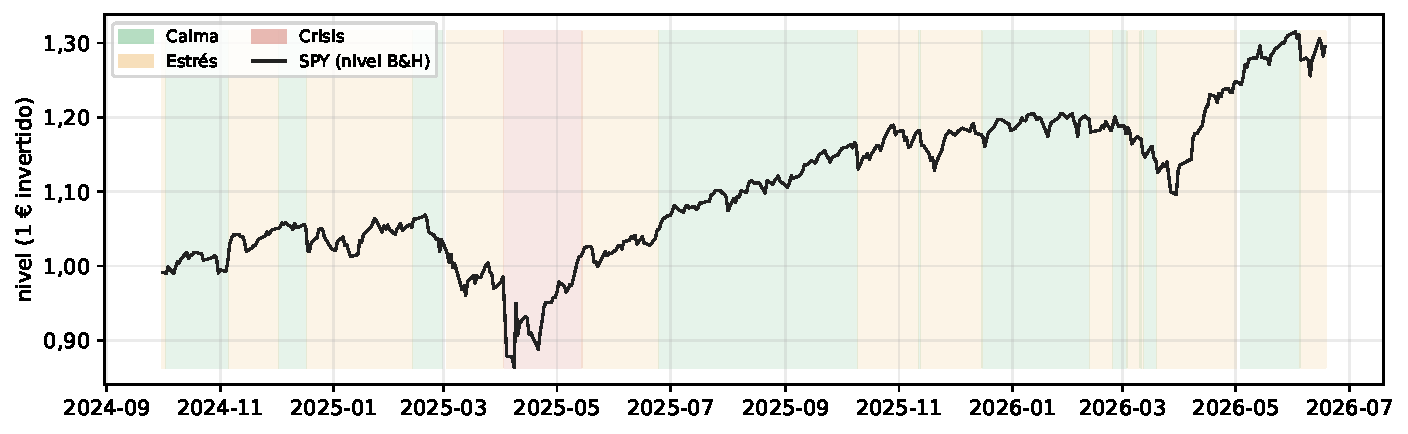
\includegraphics[width=0.74\textwidth]{figuras/cap4_regimenes_spy}
\caption{Regímenes del HMM ($K = 3$) sobre el precio de SPY en el periodo de evaluación. Calma (volatilidad baja, retorno medio positivo), Estrés (intermedio) y Crisis (volatilidad alta, retorno medio negativo) ordenan por la firma del \emph{leverage effect}. El sombreado marca el régimen vigente cada día; la coincidencia régimen$\leftrightarrow$caída es contemporánea, no predictiva.}
\label{fig:mp-regimenes-spy}
\end{figure}

Los tres detectores miran ejes ortogonales de la decisión del agente. RAM lee el régimen y comprueba si la dirección de la apuesta concuerda con el estado vigente: su \emph{score} es la probabilidad que el HMM pone en que el agente apuesta contra el régimen, y dispara cuando $\mathrm{RAM}_t \ge \tau = 0{,}50$. PSA vigila con BOCPD si el agente cambia de criterio de forma estructural (Adams y MacKay 2007 \cite{adams2007}). GSO contrasta el tamaño de la posición con la volatilidad del GARCH (Bollerslev 1986 \cite{bollerslev1986}). Cuando RAM dispara, la intervención reorienta la posición al signo del régimen, fijado por un prior calibrado por activo a partir de la media del retorno de cada estado, nunca por una regla del tipo ``Crisis implica corto'' escrita a mano.

Sobre SPY actúa una sola supervisión (Tabla~\ref{tab:mp-detectores}). RAM dispara casi un tercio de los días y acierta más al intervenir que el agente al que corrige; PSA dispara dos días y GSO ninguno. El motivo es que el agente mantiene una posición casi constante sobre SPY, corta la mayor parte de los días, de modo que sus \emph{scores} de cambio y de tamaño quedan por debajo de los umbrales de calibración. PSA y GSO son detectores inertes como reglas sobre este activo, un hallazgo que registramos. La atribución de P\&L cierra la lectura: todo el rescate acumulado sale de los días en que RAM dispara, y PSA y GSO aportan exactamente cero.

\begin{table}[htbp]
\centering
\caption{Actividad de los tres detectores sobre el OOS completo de SPY ($n = 401$ días). ``Acierto'' es la fracción de direcciones correctas en los días en que el detector dispara; el P\&L de rescate es el acumulado de la intervención en esos días. PSA y GSO apenas disparan: su columna de acierto no aplica. Fuente: \texttt{spy\_intervention\_anatomy.json}.}
\label{tab:mp-detectores}
\begin{tabular}{lrrrr}
\toprule
Detector & Tasa de disparo & Acierto M8 & Acierto M5 & P\&L de rescate \\
\midrule
\textbf{RAM} (régimen) & $\mathbf{30{,}2\%}$ & $\mathbf{0{,}587}$ & $0{,}413$ & $\mathbf{+0{,}312}$ \\
PSA (cambio estructural) & $0{,}5\%$ & --- & --- & $0{,}000$ \\
GSO (volatilidad) & $0{,}0\%$ & --- & --- & $0{,}000$ \\
\bottomrule
\end{tabular}
\end{table}

Que RAM acierte al intervenir no es casualidad, y la Figura~\ref{fig:mp-scores-detectores} lo deja ver. En los días en que RAM está alto, seguir el régimen bate a seguir al agente; cuando RAM está bajo, la ventaja se diluye y la intervención no se activa. El detector funciona como una compuerta: deja pasar la decisión del agente salvo cuando choca con el régimen, y solo entonces la corrige. En SPY esa compuerta es todo el mecanismo de la regla, porque el canal de régimen es el único que se enciende.

\begin{figure}[htbp]
\centering
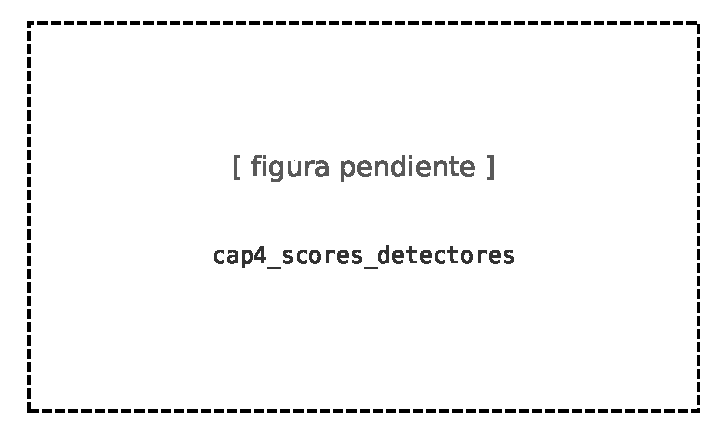
\includegraphics[width=0.74\textwidth]{figuras/cap4_scores_detectores}
\caption{Distribución de los \emph{scores} de RAM, PSA y GSO sobre el OOS de SPY, con su umbral de disparo marcado (RAM $\tau = 0{,}50$, PSA $P_{95} = 0{,}023$, GSO $P_{95} = 2{,}371$). El \emph{score} de RAM es bimodal y cruza el umbral con frecuencia; los de PSA y GSO se acumulan muy por debajo del suyo, de ahí que apenas disparen.}
\label{fig:mp-scores-detectores}
\end{figure}

La intervención puede ejecutarse de tres maneras. Puede abstenerse los días dudosos cerrando la posición, reducir el tamaño a la mitad, o reorientar la dirección al signo del régimen, el modo que llamamos \emph{override}. La Tabla~\ref{tab:mp-variantes} compara los tres sobre los días en mercado ($n = 232$). El \emph{override}, que adoptamos como modo canónico, gana en acierto y en Sharpe; abstenerse y reducir apenas se distinguen del agente sin tocar. El valor está en corregir activamente la dirección cuando choca con el régimen, no en limitarse a evitar el riesgo.

\begin{table}[htbp]
\centering
\caption{Modos de intervención de M8 sobre SPY (días en mercado, $n = 232$). El modo canónico (\emph{override}) reorienta la posición al signo del régimen; las alternativas se abstienen o reducen el tamaño. En negrita, el modo adoptado. Fuente: \texttt{spy\_intervention\_variants.json}.}
\label{tab:mp-variantes}
\begin{tabular}{lrrr}
\toprule
Modo & Accuracy & Sharpe & Capital \\
\midrule
\textbf{Override} (canónico) & $\mathbf{0{,}478}$ & $\mathbf{-0{,}46}$ & $\mathbf{0{,}94\times}$ \\
Abstención & $0{,}401$ & $-2{,}10$ & $0{,}81\times$ \\
Reducir a la mitad & $0{,}397$ & $-2{,}75$ & $0{,}75\times$ \\
M5 (agente sin tocar) & $0{,}397$ & $-3{,}07$ & $0{,}70\times$ \\
\bottomrule
\end{tabular}
\end{table}

La anatomía de esas intervenciones está en la matriz de confusión de la Figura~\ref{fig:mp-confusion-spy}: unas corrigen al agente cuando apostaba contra el régimen, otras meten ruido cuando el agente tenía razón. El saldo neto es positivo porque la intervención no es indiscriminada: crece con la discrepancia entre la apuesta del agente y el signo del régimen. Cuanto más se aleja el agente del estado del mercado, con más fuerza actúa la regla, y son justo esos días de discrepancia grande los que aportan el grueso del rescate.

\begin{figure}[htbp]
\centering
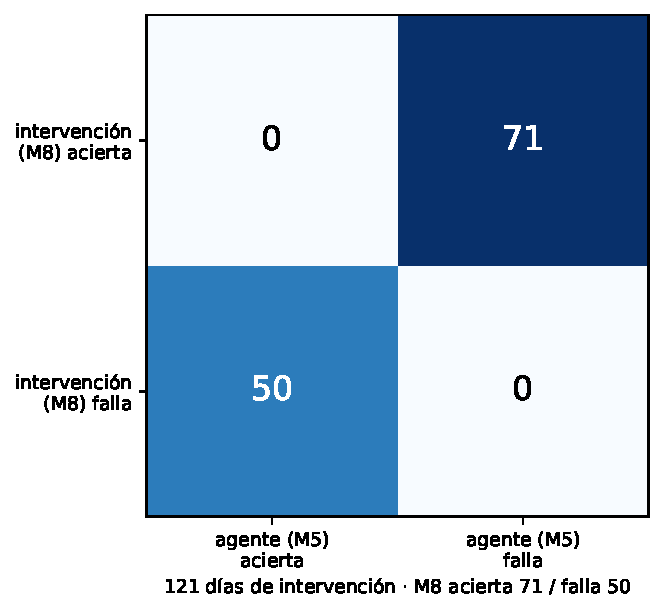
\includegraphics[width=0.7\textwidth]{figuras/cap4_confusion_spy}
\caption{Matriz de confusión de la intervención sobre SPY: dirección del agente (M5) frente a dirección tras intervenir (M8), sobre las $121$ intervenciones. La diagonal de rescate ($71$ aciertos de la intervención cuando el agente fallaba) supera a la de daño ($50$).}
\label{fig:mp-confusion-spy}
\end{figure}

\section{Comparación de las seis estrategias}
\label{sec:spy-estrategias}

Sobre el agente comparamos las seis estrategias ya introducidas en el capítulo anterior. M5 es el agente sin supervisar. M8 es la regla determinista de la intervención. M10 es el meta-learner, un ensemble de diez XGBoost sobre las veintidós características del agente y de STRATA. AutoML deja que H2O busque por reentreno entre GBM, XGBoost y su apilamiento. Las dos referencias triviales son comprar y mantener (B\&H) y la clase mayoritaria del pasado (ZeroR): marcan el listón que cualquier pretensión de habilidad debe superar. La Tabla~\ref{tab:mp-spy} las reúne sobre la ventana desplegable.

\begin{table}[htbp]
\centering
\caption{Las seis estrategias sobre SPY, ventana desplegable ($n = 251$, \texttt{signal\_lag}${}=1$). Accuracy direccional, Sharpe anualizado, máxima caída, ratio de Calmar (Young 1991 \cite{young1991}) y capital final por euro invertido. En negrita, la mejor en cada columna. Fuente: \texttt{automl\_runs/panel\_mm25\_inclGBM-XGB-SE\_AUC\_emb1\_N0-150\_step21\_kfold\_seed42.json}.}
\label{tab:mp-spy}
\begin{tabular}{lrrrrr}
\toprule
Estrategia & Accuracy & Sharpe & Máx.\ caída & Calmar & Capital \\
\midrule
\textbf{AutoML} (búsqueda H2O) & $\mathbf{0{,}574}$ & $\mathbf{+2{,}68}$ & $\mathbf{-5{,}5\%}$ & $\mathbf{6{,}93}$ & $\mathbf{1{,}38\times}$ \\
ZeroR (clase mayoritaria) & $0{,}566$ & $+2{,}21$ & $-9{,}8\%$ & $3{,}10$ & $1{,}30\times$ \\
B\&H (comprar y mantener) & $0{,}566$ & $+2{,}21$ & $-9{,}8\%$ & $3{,}10$ & $1{,}30\times$ \\
M10 (meta-learner XGBoost) & $0{,}494$ & $-0{,}60$ & $-16{,}1\%$ & $-0{,}50$ & $0{,}92\times$ \\
M8 (regla STRATA) & $0{,}442$ & $-0{,}46$ & $-15{,}2\%$ & $-0{,}39$ & $0{,}94\times$ \\
M5 (agente solo) & $0{,}366$ & $-3{,}07$ & $-30{,}2\%$ & $-1{,}00$ & $0{,}70\times$ \\
\bottomrule
\end{tabular}
\end{table}

Leída de abajo arriba, podemos decir cada capa rescata a la anterior. La regla recupera al agente y le recorta a la mitad la máxima caída; el meta-learner sube otro escalón en accuracy; AutoML llega arriba y gana en todas las columnas, también a las dos triviales. El rescate es significativo en los tres casos, contrastado con el McNemar pareado sobre los aciertos diarios frente al agente (McNemar 1947 \cite{mcnemar1947}). Los tres rescatan al agente, y el rescate aguanta el test.

La victoria sobre la trivial necesita un matiz. El mismo McNemar de AutoML frente a ZeroR no separa a las dos: no hay potencia en una ventana de doscientos cincuenta días. La ventaja de AutoML sobre el mercado pasivo es real en punto pero nominal en significancia, y tiene una explicación económica: SPY es mayormente beta de mercado, el periodo de evaluación fue alcista, e ir largo capturó esa subida. La Figura~\ref{fig:mp-equity-spy} hace visible la diferencia, y el Sharpe deflactado (López de Prado 2018 \cite{lopezdeprado2018}; Bailey y López de Prado 2014 \cite{bailey2014}) la pone en contexto. El DSR confirma esa lectura: solo el de AutoML se acerca a uno, mientras los de M10 y el agente quedan pegados a cero. AutoML es el único de los modelos cuyo Sharpe sobrevive al ajuste por número de pruebas.

\begin{figure}[htbp]
\centering
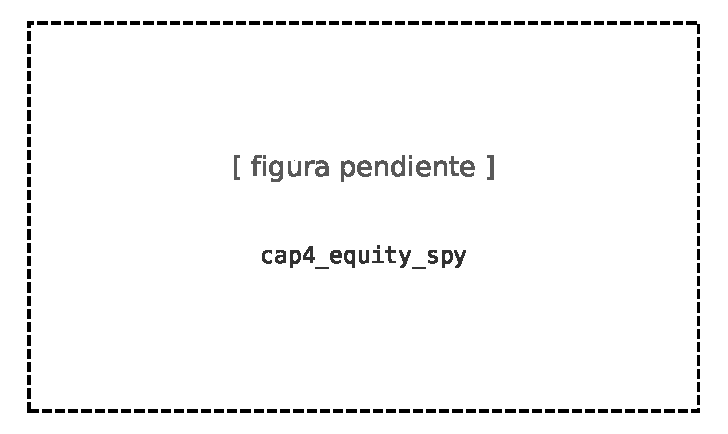
\includegraphics[width=0.74\textwidth]{figuras/cap4_equity_spy}
\caption{Curvas de capital de las seis estrategias sobre SPY (ventana desplegable, $n = 251$ días, un euro inicial). AutoML (línea destacada) supera a las dos referencias triviales en Sharpe ($+2{,}68$ frente a $+2{,}21$), en máxima caída ($-5{,}5\%$ frente a $-9{,}8\%$) y en capital final ($1{,}38\times$ frente a $1{,}30\times$); el agente solo (M5) termina en $0{,}70\times$. La ventaja sobre la trivial es nominal (McNemar AutoML vs ZeroR $p = 0{,}90$).}
\label{fig:mp-equity-spy}
\end{figure}

Sobre un único activo, el intervalo de confianza del $\Delta$Sharpe de la regla frente al agente cruza el cero. El resultado en riesgo que no alcanza significancia a este nivel, lo comprobamos en una muestra mayor de activos en el siguiente capítulo.

\section{El rescate sobre SPY}
\label{sec:spy-rescate}

Ya vimos que sobre SPY el régimen (Sección~\ref{sec:spy-anatomia}) es el único que rescata. La preguna que nos queda por responder es: ¿usa de verdad el aprendiz las señales de STRATA, o gana por otro lado? La ablación lo responde. Al quitar PSA y GSO de las características, la accuracy de AutoML baja (Tabla~\ref{tab:mp-ablacion}): aunque PSA y GSO casi no disparen como reglas, sus \emph{scores} continuos informan al modelo. Las características de Shapley (Lundberg y Lee 2017 \cite{lundberg2017}) lo confirman, y aquí etiquetamos cada cuota con su modelo y su ventana porque no son el mismo objeto. Sobre el ensemble M10 ($n = 251$), la cuota de las features de STRATA es $0{,}71$. Sobre el \emph{leader} de AutoML ($n = 401$, otro modelo y otra ventana), es $0{,}565$ por árbol y $0{,}564$ por permutación. Las dos cuotas superan la mitad y colocan los detectores por delante de las características del propio agente.

Ya vimos que sobre SPY el régimen (Sección~\ref{sec:spy-anatomia}) es el único que rescata. La pregunta que nos queda por responder es: ¿usa de verdad el aprendiz las señales de STRATA, o gana por otro lado? La ablación lo responde. Quitamos PSA y GSO de las características y reentrenamos: la accuracy de AutoML baja (Tabla~\ref{tab:mp-ablacion}). Aunque esos dos detectores casi nunca disparen como reglas, sus \emph{scores} continuos llevan información que el modelo aprovecha porque sin ellos rinde peor.

Los valores de Shapley (Lundberg y Lee 2017 \cite{lundberg2017}) lo confirman desde otro ángulo: reparten la importancia total del modelo entre las quince características del agente y las siete de STRATA. Aunque STRATA aporta solo siete de las veintidós, se lleva más de la mitad del peso. Damos la cuota etiquetada con su modelo y su ventana, porque no son el mismo objeto: sobre el ensemble M10 (ventana desplegable, $n = 251$) vale $0{,}71$; sobre el \emph{leader} de AutoML ($n = 401$, otro modelo) vale $0{,}565$ por árbol y $0{,}564$ por permutación, dos cálculos distintos que coinciden. En todos los casos supera la mitad: el aprendiz coloca los detectores por delante de las características del propio agente. Las dos pruebas apuntan a lo mismo, ablación y atribución: el aprendiz sí se apoya en STRATA.


\begin{table}[htbp]
\centering
\caption{Ablación de detectores sobre SPY (ventana desplegable, $n = 251$). El conjunto canónico usa las veintidós características; ``sin PSA+GSO'' deja solo el canal de régimen entre los detectores. AutoML degrada al quitar PSA+GSO, prueba de que usa sus \emph{scores}. Fuente: \texttt{automl\_ablation\_detectors.json}, \texttt{detector\_ablation\_panel.json}.}
\label{tab:mp-ablacion}
\begin{tabular}{lrr}
\toprule
Conjunto de características & Accuracy AutoML & Accuracy M10 \\
\midrule
\textbf{ALL22} (canónico) & $\mathbf{0{,}574}$ & $0{,}494$ \\
sin PSA+GSO & $0{,}550$ & $0{,}514$ \\
\bottomrule
\end{tabular}
\end{table}


La objeción más natural es que los umbrales se eligieran para que el resultado saliera bien. El barrido completo lo descarta (Figura~\ref{fig:mp-sensibilidad}): la accuracy apenas se mueve alrededor del valor canónico, ni al variar el umbral $\tau$ de RAM en M8 ni el umbral de decisión del meta-learner. El resultado no cuelga de un punto afortunado, sino que descansa sobre una meseta estable; es lo contrario de un ajuste fino al periodo de evaluación y es lo que nos protege de la sospecha de sobreajuste.


\begin{figure}[htbp]
\centering
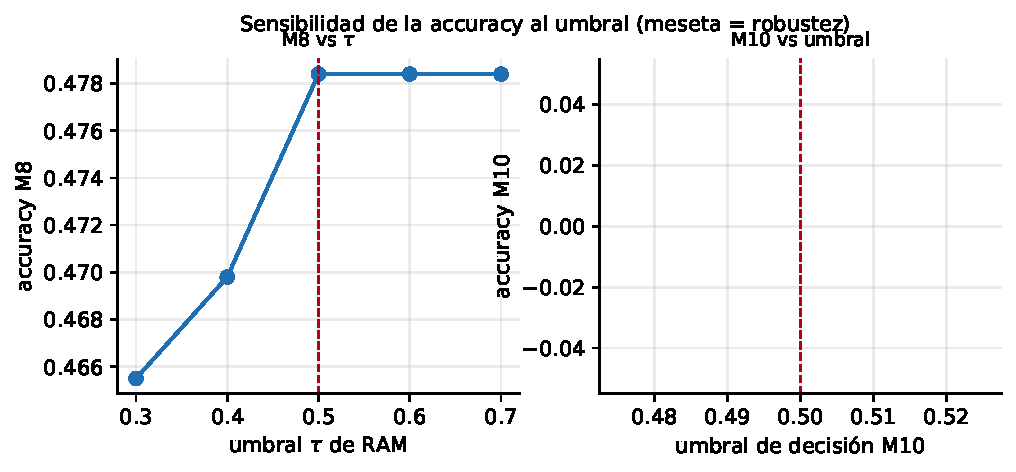
\includegraphics[width=0.74\textwidth]{figuras/cap4_sensibilidad_umbrales}
\caption{Sensibilidad de la accuracy al umbral de decisión sobre SPY: M8 frente a $\tau$ del detector RAM y M10 frente a su umbral de probabilidad. Las dos curvas son planas en una meseta alrededor del valor canónico (marcado), señal de robustez y no de ajuste a un punto.}
\label{fig:mp-sensibilidad}
\end{figure}

Para concluir, sobre SPY el mecanismo es transparente y el agente, sin supervisión, pierde con holgura. La intervención por régimen lo corrige de forma significativa, la derivada aprendida supera a la trivial en este punto apoyándose en las señales de STRATA, y todo descansa sobre una meseta robusta de umbrales. A nivel de un único activo, sin embargo, la corrección de riesgo no alcanza significancia y la victoria sobre la trivial es nominal. Queda la pregunta que enfoca el resto del trabajo: ¿se sostiene el rescate fuera de SPY? El panel de diez activos es el siguiente paso.

\chapter{Validación sobre el panel de diez activos}
\label{cap:panel}

% Fuente única de cifras: notebooks/STRATA_marco_practico.ipynb (panel canónico de 10) y sus JSON en
% outputs/experiments/. Toda cifra trazada a su JSON en el caption de su tabla.

En SPY STRATA rescató al agente, pero sobre un único activo el intervalo de confianza del $\Delta$Sharpe del rescate cruzaba el cero: la corrección apuntaba bien, mas no se separaba del cero en solitario. La prueba dura vive en el panel: diez activos (SPY, QQQ, XLF, DIA, XLK, XLE, ROKU, SMCI, MARA, UNG), elegidos por su naturaleza para cubrir distintos grados de \emph{leverage effect}. Sobre ellos repetimos toda la cadena de SPY, agregamos los resultados y buscamos el patrón que ordena el rescate. Al apilar el panel, el rescate de riesgo que en un activo no alcanzaba significancia la alcanza.

\section{El rescate en el panel}
\label{sec:panel-agregado}

El problema que vimos en SPY no es de SPY. A través del panel el agente pierde y acierta menos de la mitad de las direcciones con regularidad: queda por debajo de $0{,}5$ en siete de los diez activos, y allí donde lo supera lo hace por poco y con un Sharpe pobre. El agente solo no es una estrategia, es el punto de partida que STRATA tiene que corregir.

\subsection{La compuerta de régimen y la activación de detectores}
\label{sec:panel-gate}

Los tres detectores no se encienden por igual. RAM domina en todas partes, igual que en SPY; PSA y GSO disparan poco, porque el agente mantiene posiciones casi constantes y sus \emph{scores} rara vez cruzan los umbrales. La Tabla~\ref{tab:mp-gate} recoge la tasa de intervención por activo y la compuerta de régimen: en los días en que RAM dispara, seguir el signo del régimen bate a seguir al agente en \textbf{seis de los diez} activos. La intervención no se reparte al azar: su tasa crece con la discrepancia entre la apuesta del agente y el signo del régimen, y esa relación es casi recta (Figura~\ref{fig:mp-gate-ram}; activo a activo en la Figura~\ref{fig:mp-activacion-panel} del Anexo~\ref{anx:figuras}).

\begin{table}[htbp]
\centering
\caption{Activación de RAM y compuerta de régimen por activo (OOS completo del panel). ``Tasa interv.'' es la fracción de días en que RAM dispara; ``discrepancia'' es la fracción de días en que la apuesta del agente choca con el signo del régimen; ``gate RAM'' indica si, en los días de disparo, seguir el régimen bate a seguir al agente. PSA y GSO disparan de forma marginal en todo el panel.}
\label{tab:mp-gate}
\begin{tabular}{lrrl}
\toprule
Activo & Tasa interv.\ (RAM) & Discrepancia agente$\leftrightarrow$régimen & Gate RAM \\
\midrule
SPY  & $0{,}302$ & $0{,}601$ & régimen $>$ agente \\
QQQ  & $0{,}197$ & $0{,}526$ & régimen $>$ agente \\
XLF  & $0{,}549$ & $0{,}720$ & régimen $>$ agente \\
DIA  & $0{,}343$ & $0{,}603$ & agente $>$ régimen \\
XLK  & $0{,}095$ & $0{,}372$ & agente $>$ régimen \\
XLE  & $0{,}596$ & $0{,}781$ & régimen $>$ agente \\
ROKU & $0{,}710$ & $0{,}823$ & régimen $>$ agente \\
SMCI & $0{,}018$ & $0{,}120$ & régimen $>$ agente \\
MARA & $0{,}415$ & $0{,}666$ & agente $>$ régimen \\
UNG  & $0{,}078$ & $0{,}169$ & agente $>$ régimen \\
\bottomrule
\end{tabular}
\end{table}

\begin{figure}[htbp]
\centering
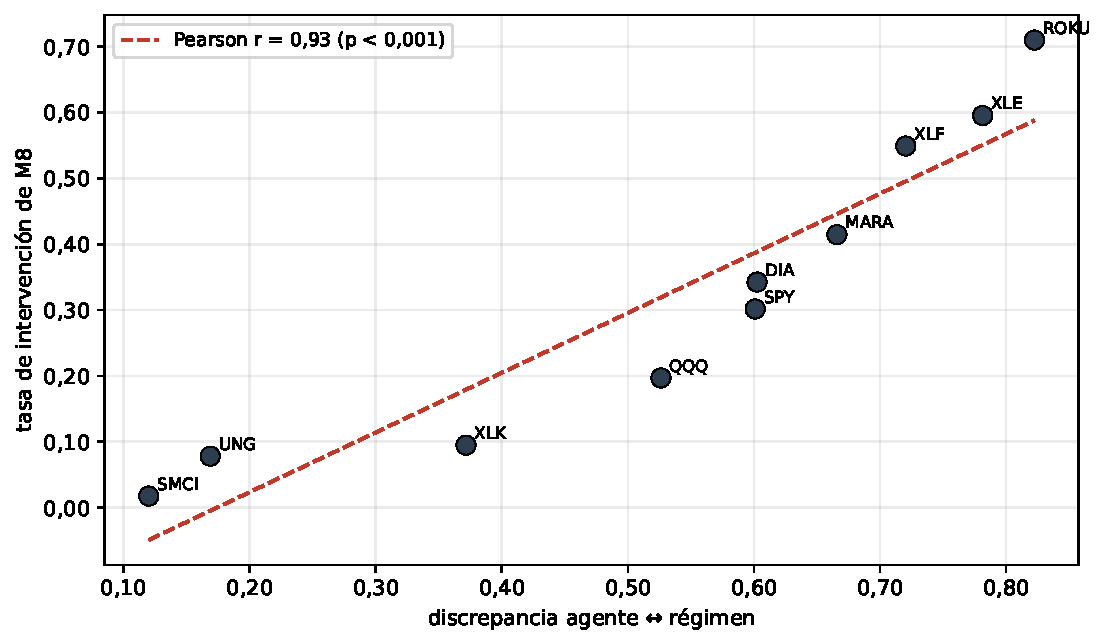
\includegraphics[width=0.60\textwidth]{figuras/cap4_gate_ram}
\caption{Compuerta de régimen sobre el panel: tasa de intervención de RAM frente a la discrepancia media entre la apuesta del agente y el signo del régimen, un punto por activo. La relación es casi recta (Pearson $r = 0{,}93$, $p < 0{,}001$): cuanto más se aleja el agente del estado del mercado, con más frecuencia actúa la regla.}
\label{fig:mp-gate-ram}
\end{figure}

\subsection{Accuracy por activo: dónde se bate a la trivial}
\label{sec:panel-accuracy}

La Tabla~\ref{tab:mp-accuracy} cruza los diez activos con las seis estrategias en accuracy direccional. La mejor derivada de STRATA mejora al agente en los \textbf{diez de diez} activos, con una mejora media de $+0{,}086$; en ninguno supervisar lo empeora. Qué estrategia gana cambia de un activo a otro, coherente con la idea de dos capas: en unos manda la regla, en otros el aprendiz, según la naturaleza del activo.

\begin{table}[htbp]
\centering
\caption{Accuracy direccional por activo y estrategia (ventana desplegable, \texttt{signal\_lag}${}=1$). En negrita, la mejor derivada de STRATA (M8/M10/AutoML) cuando supera a las dos referencias triviales (ZeroR y B\&H) en ese activo. ZeroR y B\&H comparten valor salvo cuando difieren.}
\label{tab:mp-accuracy}
\begin{tabular}{lrrrrrr}
\toprule
Activo & M5 & M8 & M10 & AutoML & ZeroR & B\&H \\
\midrule
SPY  & $0{,}366$ & $0{,}442$ & $0{,}494$ & $\mathbf{0{,}574}$ & $0{,}566$ & $0{,}566$ \\
QQQ  & $0{,}418$ & $0{,}486$ & $0{,}522$ & $0{,}534$ & $0{,}590$ & $0{,}590$ \\
XLF  & $0{,}429$ & $0{,}502$ & $0{,}526$ & $0{,}510$ & $0{,}538$ & $0{,}538$ \\
DIA  & $0{,}440$ & $0{,}484$ & $0{,}468$ & $0{,}520$ & $0{,}552$ & $0{,}556$ \\
XLK  & $0{,}510$ & $0{,}470$ & $0{,}542$ & $0{,}590$ & $0{,}641$ & $0{,}641$ \\
XLE  & $0{,}448$ & $0{,}528$ & $0{,}508$ & $0{,}532$ & $0{,}565$ & $0{,}565$ \\
ROKU & $0{,}444$ & $0{,}528$ & $0{,}508$ & $0{,}544$ & $0{,}548$ & $0{,}548$ \\
SMCI & $0{,}484$ & $0{,}496$ & $\mathbf{0{,}552}$ & $0{,}472$ & $0{,}516$ & $0{,}484$ \\
MARA & $0{,}528$ & $0{,}528$ & $0{,}532$ & $\mathbf{0{,}544}$ & $0{,}532$ & $0{,}468$ \\
UNG  & $0{,}510$ & $0{,}502$ & $\mathbf{0{,}518}$ & $0{,}482$ & $0{,}449$ & $0{,}486$ \\
\bottomrule
\end{tabular}
\end{table}

En cuatro activos una derivada de STRATA supera en punto a las dos referencias triviales a la vez: SPY y MARA por AutoML, SMCI y UNG por M10 (Tabla~\ref{tab:mp-accuracy}, celdas en negrita). En los seis restantes la trivial aguanta; en índices muy direccionales como XLK la clase mayoritaria del pasado se va por encima de $0{,}64$ y ninguna derivada se le acerca.

Estas victorias son reales en punto y nominales. Con del orden de doscientos cincuenta días por activo y una ganadora que cambia de un activo a otro, se eligen a posteriori, y ninguna bate a ZeroR con significancia: el McNemar pareado de AutoML frente a ZeroR sobre SPY da $p = 0{,}90$, sin potencia para separarlos. El mapa completo está en la Figura~\ref{fig:mp-heatmap}, con solo cuatro celdas de derivada del lado bueno, y el reparto de aciertos y fallos en la Figura~\ref{fig:anx-confusion-panel}. La prueba que sí sobrevive a un test vive en el riesgo, no en la accuracy frente a la trivial.

\begin{figure}[htbp]
\centering
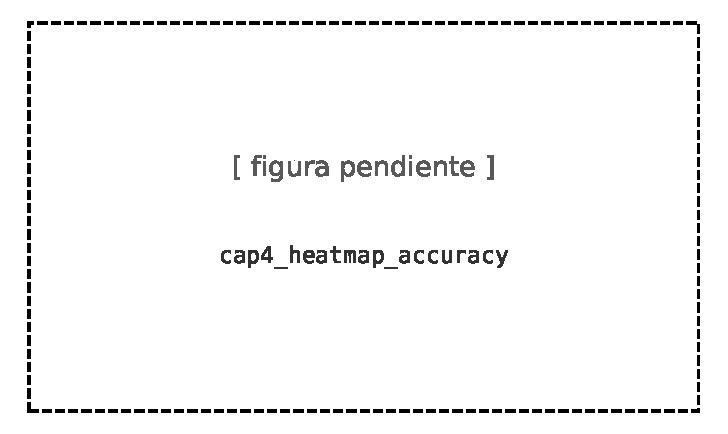
\includegraphics[width=0.62\textwidth]{figuras/cap4_heatmap_accuracy}
\caption{Mapa de calor de la accuracy direccional por activo (filas) y estrategia (columnas), centrado en $0{,}5$: el color mide la distancia a una referencia trivial. Verde marca accuracy por encima de la trivial del activo, rojo por debajo. La mejor derivada de STRATA supera a las dos triviales solo en SPY, SMCI, MARA y UNG; en los demás la trivial aguanta. Victorias nominales (n${}\approx 250$, a posteriori).}
\label{fig:mp-heatmap}
\end{figure}

\subsection{Pooled: el rescate en riesgo}
\label{sec:panel-pooled}

SPY mostró que el problema era de potencia, no de señal: con una muestra tan pequeña, el intervalo del $\Delta$Sharpe no se separaba del cero aunque la mejora estuviera ahí. La salida es agregar: si la supervisión rescata por el mismo mecanismo en activos distintos, apilar sus días multiplica la muestra. Apilamos los días de los diez activos (\emph{pooled-10}, $n = 2493$ días) y medimos el $\Delta$Sharpe pareado frente a M5 día a día, cada comparación sobre el mismo día y el mismo activo.

La validez del agregado depende del remuestreo. Extraer días sueltos trataría la serie como independiente, y no lo es: los retornos de días vecinos se parecen y eso estrecharía el intervalo de forma artificial. Por eso usamos el \emph{bootstrap} estacionario \cite{politis1994}, que toma tramos con inicio al azar y longitud variable de media $\sqrt{n}$; así los días vecinos viajan juntos y el intervalo recoge la dependencia temporal real.

El resultado lo reúne la Tabla~\ref{tab:mp-pooled}: las tres estrategias supervisadas dejan un $\Delta$Sharpe positivo cuyo límite inferior queda por encima de cero, la afirmación que SPY no sostenía en solitario.

\begin{table}[htbp]
\centering
\caption{Rescate en riesgo agregado (\emph{pooled-10}, $n = 2493$ días): $\Delta$Sharpe de cada estrategia supervisada frente al agente M5, con intervalo de confianza al $95\%$ por \emph{bootstrap} estacionario de bloque medio $\sqrt{n}$ (Politis y Romano 1994). Los tres intervalos excluyen el cero.}
\label{tab:mp-pooled}
\begin{tabular}{lrc}
\toprule
Estrategia & $\Delta$Sharpe & IC$_{95}$ \\
\midrule
M8 (regla)            & $+0{,}60$ & $[0{,}05,\ 1{,}22]$ \\
M10 (meta-learner)    & $+1{,}12$ & $[0{,}39,\ 1{,}84]$ \\
\textbf{AutoML} (H2O) & $\mathbf{+1{,}08}$ & $[0{,}40,\ 1{,}85]$ \\
\bottomrule
\end{tabular}
\end{table}

Hay un orden entre ellas (Figura~\ref{fig:mp-forest}): la regla queda con su límite inferior pegado al borde mientras los dos aprendices guardan holgura, de modo que el rescate de riesgo es más firme en los aprendices, aunque ninguno cruza el cero.

\begin{figure}[htbp]
\centering
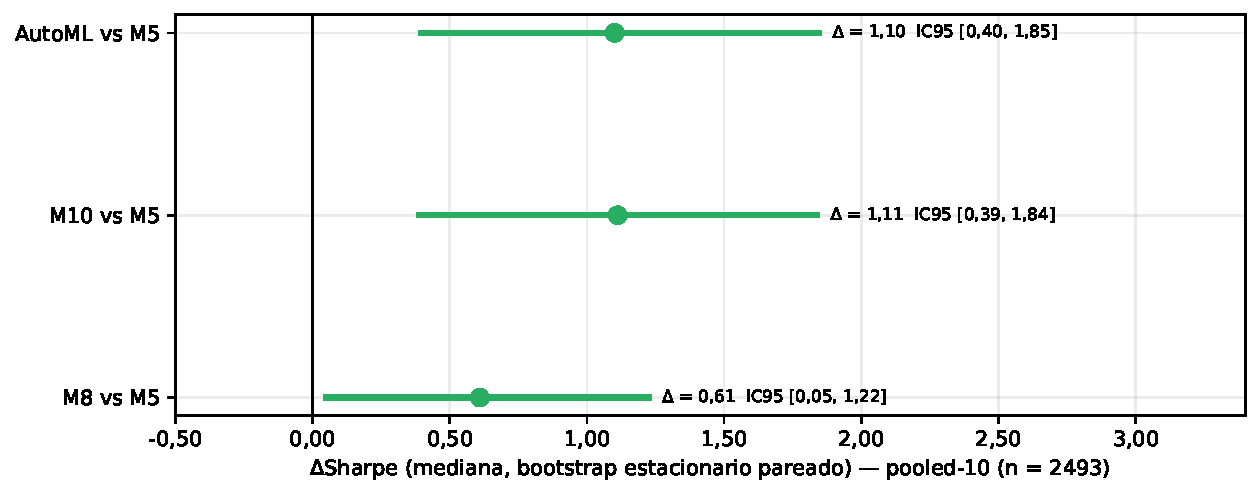
\includegraphics[width=0.60\textwidth]{figuras/cap4_forest_pooled}
\caption{Diagrama de bosque del $\Delta$Sharpe \emph{pooled-10} frente al agente M5, con intervalo al $95\%$ (\emph{bootstrap} estacionario, Politis y Romano 1994). La línea vertical marca el cero. Los tres intervalos excluyen el cero; la regla M8 con el límite inferior más cerca del borde y los aprendices M10 y AutoML con más holgura.}
\label{fig:mp-forest}
\end{figure}

El agregado tiene un matiz. El \emph{pooled} apila los días de los diez activos como si fueran independientes, y no lo son: la correlación cruzada entre índices es alta (SPY y QQQ por encima de $0{,}9$), lo que reduce el tamaño de muestra efectivo y deja el intervalo algo optimista. El bloque medio $\sqrt{n}$ del \emph{bootstrap} amortigua parte del efecto al remuestrear bloques contiguos.

En la economía, una derivada de STRATA bate al pasivo en Sharpe en cuatro activos: SPY, SMCI, MARA y UNG (Figura~\ref{fig:mp-equity-panel} del Anexo~\ref{anx:figuras}). En SMCI, MARA y UNG el pasivo pierde o ronda el cero y la derivada saca un Sharpe positivo yendo defensiva, sin estar largo en una subida. En SPY el periodo fue alcista y el activo es mayormente beta de mercado, así que el Sharpe positivo refleja sobre todo la exposición al índice.

\subsection{Equivalencia: el aprendiz redescubre STRATA y bate a la regla}
\label{sec:panel-tost}

Si el aprendiz mejora a la regla, ¿de qué se alimenta? Se apoya en los detectores de STRATA. Las cuotas de Shapley \cite{lundberg2017} miden cuánto del juicio del aprendiz descansa en cada bloque de características; la de las features de STRATA supera la mitad en los \textbf{diez de diez} activos, con una media de $0{,}66$. El aprendiz no inventa una señal nueva: redescubre los detectores que diseñamos a mano y los pondera por encima de las características del agente.

Que se apoye en STRATA no quiere decir que solo replique la regla. El contraste lo da el TOST de Schuirmann \cite{schuirmann1987}: al revés que un test de superioridad, parte de que las dos estrategias son distintas y solo concede equivalencia si la evidencia de parecido es fuerte, exigiendo rechazar por los dos lados a la vez. La Tabla~\ref{tab:mp-tost} lo aplica al aprendiz frente a la regla M8. En accuracy no hay equivalencia y el desempate va para el aprendiz: M10 y AutoML superan a la regla con un intervalo al $90\%$ por encima de cero. En Sharpe es no concluyente, indistinguibles en riesgo. El mecanismo es claro: la regla M8 es una compuerta fija sobre el régimen, mientras el aprendiz modela interacciones no lineales entre régimen y agente que la regla no alcanza, y de ahí saca el punto extra de accuracy.

\begin{table}[htbp]
\centering
\caption{TOST del aprendiz frente a la regla M8 (Schuirmann 1987) y cuota de Shapley de las features de STRATA por activo (Lundberg y Lee 2017). En accuracy el aprendiz supera a la regla (intervalo al $90\%$ por encima de cero); en Sharpe el test es no concluyente (indistinguibles). La cuota SHAP de STRATA supera $0{,}5$ en los diez activos.}
\label{tab:mp-tost}
\begin{tabular}{lccc}
\toprule
Comparación & $\Delta$accuracy (IC$_{90}$) & TOST Sharpe & Cuota SHAP STRATA \\
\midrule
M10 vs M8     & $+0{,}021\ [+0{,}001,\ +0{,}039]$ & no concluyente & \multirow{2}{*}{$>0{,}5$ en $10/10$ (media $0{,}66$)} \\
AutoML vs M8  & $+0{,}034\ [+0{,}010,\ +0{,}056]$ & no concluyente & \\
\bottomrule
\end{tabular}
\end{table}

El aprendiz deja, entonces, dos hechos atados con su test: se apoya en STRATA, con cuota SHAP mayoritaria en los diez activos, y bate modestamente a la regla en accuracy sin distinguirse de ella en riesgo (diagrama $2\times 2$ en la Figura~\ref{fig:mp-tost} del Anexo~\ref{anx:figuras}). La Tabla~\ref{tab:mp-capas} cierra el reparto sobre el panel (su lectura por detector, en la Figura~\ref{fig:mp-capas} del Anexo~\ref{anx:figuras}).

\begin{table}[htbp]
\centering
\caption{Atribución por capa sobre el panel de diez activos. La regla (M8) aporta el rescate de riesgo, con todo su P\&L de intervención concentrado en el canal de régimen (RAM, Figura~\ref{fig:mp-capas}); nunca lidera en accuracy. El aprendiz (M10/AutoML) aporta el rescate de accuracy y no lidera el riesgo en exclusiva. El capital final es sobre la ventana desplegable de SPY partiendo de un euro; el agente solo termina en $0{,}70\times$. $\Delta$Sharpe pooled frente al agente, IC$_{95}$ por bootstrap estacionario.}
\label{tab:mp-capas}
\begin{tabular}{lll}
\toprule
 & Regla (M8) & Aprendiz (M10/AutoML) \\
\midrule
Eje que rescata & riesgo & accuracy \\
$\Delta$Sharpe pooled vs M5 & $\mathbf{+0{,}60}$ $[0{,}05,\,1{,}22]$ & $+1{,}12$ / $+1{,}08$ \\
Capital final sobre SPY & $0{,}94\times$ & $0{,}92\times$ / $1{,}38\times$ \\
Lidera en accuracy & $0/10$ & $\mathbf{10/10}$ \\
Significancia accuracy (McNemar) & al borde & significativa \\
\bottomrule
\end{tabular}
\end{table}

\subsection{Complementariedad: bull, bear y diferencia en diferencias}
\label{sec:panel-regimen}

Un rescate que solo funcionara en mercado alcista no serviría de mucho, porque el régimen peligroso es el bajista. Partimos el panel por régimen y medimos el rescate en cada mitad con el McNemar pooled de la estrategia superior frente al agente, corrigiendo por Holm las comparaciones múltiples \cite{holm1979}. El rescate aparece en los dos (Tabla~\ref{tab:mp-regimen}): en alcista los dos aprendices rescatan de forma significativa y la regla M8 queda al borde; en bajista los tres pasan, con la regla ya holgadamente dentro.

\begin{table}[htbp]
\centering
\caption{Rescate por régimen (McNemar pooled de la estrategia superior frente a M5, $p$ corregido por Holm 1979) y complementariedad de los aprendices (DiD). El rescate es significativo en alcista y en bajista. El DiD contrasta el $\Delta\Delta$Sharpe entre aprendices y regímenes: M10 rescata más en alcista, AutoML más en bajista.}
\label{tab:mp-regimen}
\begin{tabular}{lccc}
\toprule
 & M8 & M10 & AutoML \\
\midrule
McNemar alcista (Holm $p$) & $0{,}099$ & $0{,}0076$ & $0{,}0092$ \\
McNemar bajista (Holm $p$) & $0{,}0092$ & $0{,}0268$ & $0{,}0017$ \\
\midrule
\multicolumn{4}{l}{DiD complementariedad: $\Delta\Delta$Sharpe pooled $= +1{,}37$, IC$_{95}\,[0{,}20,\ 2{,}60]$, $p = 0{,}008$} \\
\bottomrule
\end{tabular}
\end{table}

Los dos aprendices no rescatan igual en cada régimen: M10 protege más en alcista, AutoML más en bajista (Figura~\ref{fig:mp-did} del Anexo~\ref{anx:figuras}). Para contrastar si ese reparto es real construimos un test de diferencia en diferencias, pre-registrado: comparamos la diferencia de $\Delta$Sharpe entre los dos aprendices entre los dos regímenes, de modo que cualquier efecto común se cancela y queda solo la complementariedad. El $\Delta\Delta$Sharpe pooled excluye el cero (Tabla~\ref{tab:mp-regimen}): la complementariedad por régimen es significativa sobre el panel. El rescate en acierto también lo es en los dos regímenes (Figura~\ref{fig:anx-mcnemar}).

Queda la falsación pre-registrada, y el panel la resuelve. En SPY solo, en régimen bajista la regla M8 se invierte: sobre sus cincuenta días bajistas el $\Delta$Sharpe es $-1{,}49$, la regla daña en vez de rescatar. Sobre los diez activos el rescate por régimen es significativo en bajista, y la complementariedad DiD lo es en \emph{pooled} pero no en SPY aislado: el fenómeno es de panel. Queda el porqué del reparto por activo, y la respuesta está en la naturaleza del activo.

\section{El patrón: ley del leverage y clustering}
\label{sec:panel-patron}

% Clustering = EXPLORATORIO (n=10).

La sección anterior deja un hecho sin explicar: qué canal rescata cada activo cambia de uno a otro. La propiedad que ordena el rescate del aprendiz resulta ser el \emph{leverage effect}, y un clustering sin etiquetas recupera los mismos grupos que esa propiedad marca. Sobre diez activos esto es un patrón, no un teorema.

\subsection{La ley del \emph{leverage}}
\label{sec:panel-ley}

Los diez activos no son intercambiables (Figura~\ref{fig:mp-naturaleza} del Anexo~\ref{anx:figuras}): difieren en \emph{leverage}, en cuánta Crisis viven, en el sesgo del agente y en volatilidad.

El rescate del aprendiz en accuracy escala con el \emph{leverage effect} del activo. Medimos el rescate como $\max(\mathrm{M10},\mathrm{AutoML}) - \mathrm{M5}$ en accuracy y la naturaleza del activo con la correlación de Black, $\mathrm{leverage\_corr} = \operatorname{corr}(r_t,\ \mathrm{RV}^{21}_{t+1} - \mathrm{RV}^{21}_t)$, negativa cuando una caída eleva la volatilidad de mañana (\cite{black1976}; \cite{christie1982}).

Las dos magnitudes corren juntas: cuanto más negativo es el \emph{leverage} de un activo, más rescata el aprendiz en accuracy (Tabla~\ref{tab:mp-ley}, Figura~\ref{fig:mp-scatter}). La siguen nueve de los diez activos; ROKU es la única excepción, con \emph{leverage} casi nulo y un rescate alto. Hay un mecanismo detrás, el mismo de la Sección~\ref{sec:panel-pooled}: cuando el régimen es direccional, la regla disciplina el riesgo y al aprendiz le queda margen para afinar la dirección; cuando el régimen no informa el signo, el aprendiz rescata por otra vía y la ganancia se estrecha.

Con diez activos el contraste tiene poca potencia, de modo que lo presentamos como tendencia significativa al $\alpha = 0{,}10$ fijado por adelantado, no como ley exacta (Pearson $r = -0{,}56$, $p = 0{,}093$). Y su alcance es acotado: ordena el rescate del \emph{aprendiz}, no el de la regla, que no se deja predecir por la naturaleza del activo.

\begin{table}[htbp]
\centering
\caption{Ley del \emph{leverage}: correlación de Black y rescate del aprendiz por activo (panel de diez), ordenados por \emph{leverage} creciente. Rescate ${}= \max(\mathrm{M10},\mathrm{AutoML}) - \mathrm{M5}$ en accuracy. Nueve de los diez siguen la tendencia (a más \emph{leverage} negativo, más rescate); ROKU es la excepción. Sobre los diez: Pearson $r = -0{,}56$ ($p = 0{,}093$), Spearman $\rho = -0{,}59$ ($p = 0{,}074$); tendencia significativa al $\alpha = 0{,}10$ pre-registrado.}
\label{tab:mp-ley}
\begin{tabular}{lrrl}
\toprule
Activo & \texttt{leverage\_corr} & Rescate aprendiz & \\
\midrule
DIA  & $-0{,}112$ & $0{,}080$ & \\
SPY  & $-0{,}110$ & $0{,}207$ & \\
QQQ  & $-0{,}092$ & $0{,}116$ & \\
XLF  & $-0{,}091$ & $0{,}097$ & \\
XLE  & $-0{,}089$ & $0{,}085$ & \\
XLK  & $-0{,}086$ & $0{,}080$ & \\
MARA & $-0{,}059$ & $0{,}016$ & \\
SMCI & $-0{,}004$ & $0{,}068$ & \\
ROKU & $+0{,}003$ & $0{,}100$ & (excepción) \\
UNG  & $+0{,}041$ & $0{,}008$ & \\
\midrule
\emph{leverage} fuerte (media) & & $0{,}097$ & \\
\emph{leverage} débil (media)  & & $0{,}059$ & \\
\bottomrule
\end{tabular}
\end{table}

\begin{figure}[htbp]
\centering
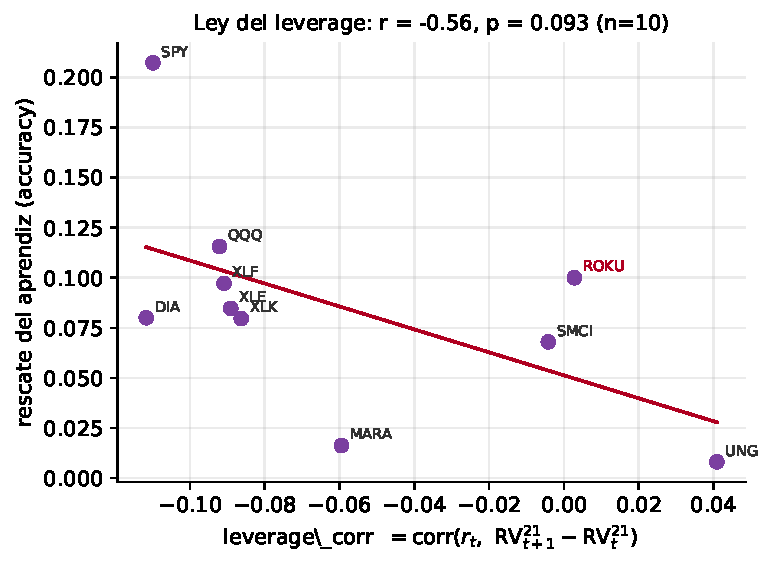
\includegraphics[width=0.60\textwidth]{figuras/cap4_scatter_leverage}
\caption{Rescate del aprendiz en accuracy frente al \emph{leverage} del activo, sobre los diez. Cada punto es un activo; el eje horizontal es la correlación de Black $\operatorname{corr}(r_t,\ \mathrm{RV}^{21}_{t+1}-\mathrm{RV}^{21}_t)$, el vertical el rescate $\max(\mathrm{M10},\mathrm{AutoML}) - \mathrm{M5}$. La recta de regresión baja con el \emph{leverage}: a más \emph{leverage} negativo, más rescate (Pearson $r = -0{,}56$, $p = 0{,}093$; tendencia significativa al $\alpha = 0{,}10$ pre-registrado). Nueve de los diez la siguen; ROKU, señalado, es la excepción.}
\label{fig:mp-scatter}
\end{figure}

\subsection{Clustering: la naturaleza separa los grupos}
\label{sec:panel-clustering}

La ley del \emph{leverage} es una recta. Queda ver si la misma estructura aparece cuando no le decimos al algoritmo qué buscar. Aparece: describimos cada activo por cinco rasgos de naturaleza (\emph{leverage}, retorno medio en Crisis, fracción de días en Crisis, volatilidad OOS y sesgo direccional del agente) y lo agrupamos con cuatro métodos —$k$-medias \cite{macqueen1967,lloyd1982}, enlace de Ward \cite{ward1963}, mezcla gaussiana \cite{dempster1977} y clustering espectral \cite{ng2002spectral}— sin ver ni una métrica de rescate.

Los cuatro coinciden en una partición unánime y bien separada (Tabla~\ref{tab:mp-cluster}): con tres grupos, el índice de Rand ajustado entre cualquier par de métodos vale uno \cite{hubert1985}. Cada grupo trae asociado un canal de rescate distinto: los índices de \emph{leverage} fuerte y los volátiles, rescatados por AutoML, y los de \emph{leverage} invertido, por M10. Los perfiles de accuracy y Sharpe por grupo están en la Figura~\ref{fig:anx-grupos}.

El cierre lo da la geometría. Al proyectar la naturaleza de los diez sobre sus dos primeras componentes principales, el primer eje recupera casi exactamente el \emph{leverage} ($r = 0{,}84$ entre PC1 y \texttt{leverage\_corr}, Figura~\ref{fig:mp-pca}): sin etiquetas de rescate, el clustering ordena los activos por el mismo eje que la ley de la Sección~\ref{sec:panel-ley}. La Figura~\ref{fig:mp-casos} del Anexo~\ref{anx:figuras} lo aterriza en dos casos, XLE rescatado por el régimen y MARA por la vía del \emph{leverage} invertido.

Con diez activos esto es exploratorio: el clustering describe, no confirma. El cluster predice el \emph{tipo} de canal que rescata cada grupo, no el modelo exacto que ganará por activo, que puede cambiar dentro de un mismo grupo. Se deja para líneas futuras.

\begin{table}[htbp]
\centering
\caption{Perfil de los tres grupos del \emph{clustering} de la naturaleza de los diez activos (cinco rasgos: \emph{leverage}, retorno medio en Crisis, fracción en Crisis, volatilidad OOS, sesgo del agente): \emph{leverage} medio de cada grupo y su mejor canal de rescate. Los cuatro métodos coinciden en esta misma partición (Rand $= 1{,}0$, silueta $0{,}55$).}
\label{tab:mp-cluster}
\begin{tabular}{lrl}
\toprule
Cluster & \emph{leverage} medio & Mejor canal \\
\midrule
C0 índices (SPY, QQQ, XLF, DIA, XLK, XLE) & $-0{,}097$ & AutoML \\
C1 \emph{leverage} invertido (SMCI, UNG)  & $+0{,}018$ & M10 \\
C2 volátiles (ROKU, MARA)                 & $-0{,}028$ & AutoML \\
\bottomrule
\end{tabular}
\end{table}

\begin{figure}[htbp]
\centering
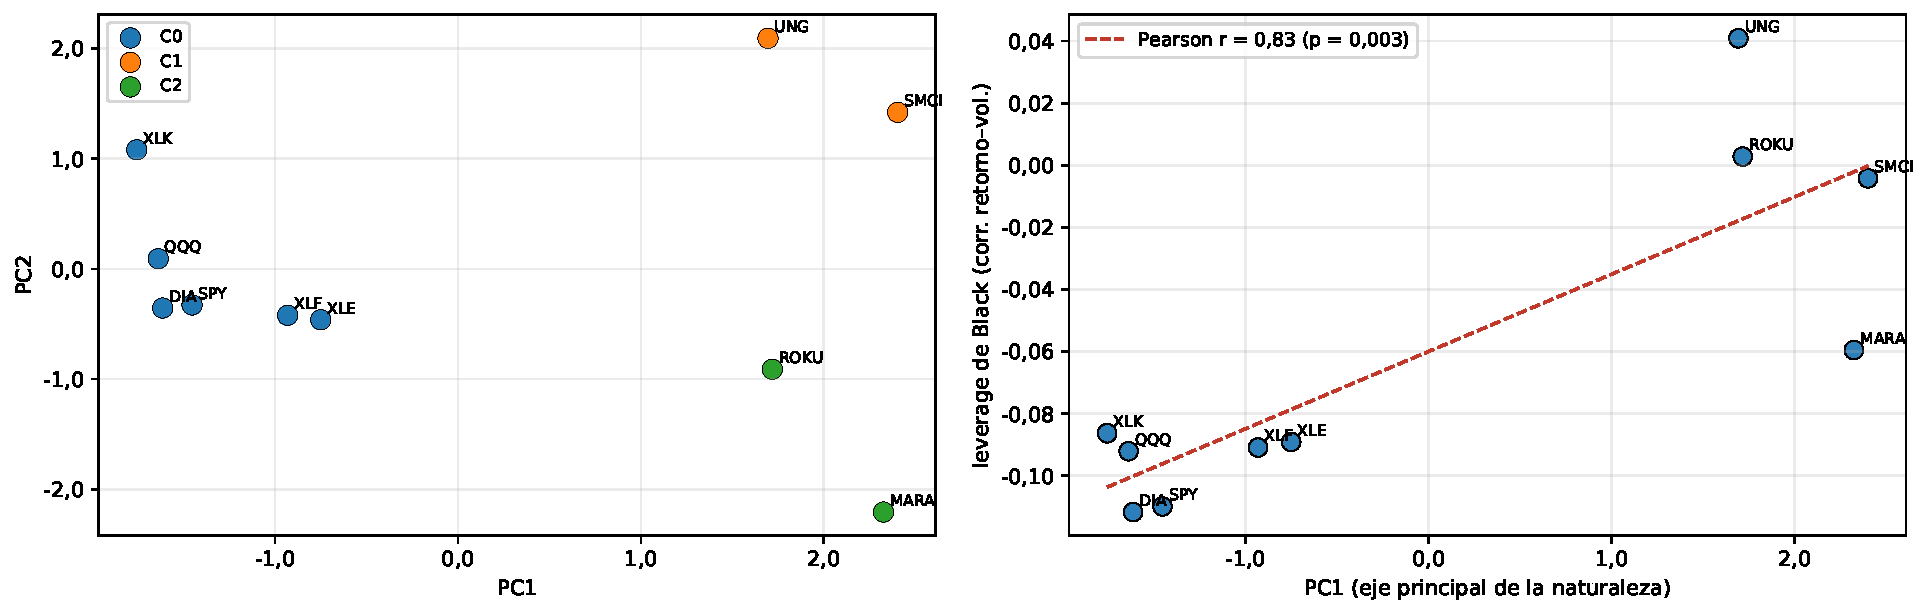
\includegraphics[width=0.60\textwidth]{figuras/cap4_pca_clusters}
\caption{Proyección de la naturaleza de los diez activos sobre sus dos primeras componentes principales. Cada punto es un activo, coloreado por su cluster ($K=3$, partición unánime de los cuatro métodos, Rand $= 1{,}0$). El primer eje recupera el \emph{leverage} ($r = 0{,}84$ entre PC1 y \texttt{leverage\_corr}): el clustering ordena los activos, sin etiquetas de rescate, por el mismo eje que la ley del \emph{leverage}. La leyenda marca el mejor canal de cada grupo (C0/C2 AutoML, C1 M10).}
\label{fig:mp-pca}
\end{figure}

\section{Robustez}
\label{sec:panel-robustez}

El rescate no depende de una elección afortunada. Se mantiene al mover la ventana de calibración de los detectores (Figura~\ref{fig:mp-robustez-calib} del Anexo~\ref{anx:figuras}) y aguanta en el panel por tres vías a la vez: la importancia de STRATA es estable en el tiempo, el rescate sobrevive a distintas particiones y se sostiene partido por régimen (Figura~\ref{fig:mp-robustez-panel} del Anexo~\ref{anx:figuras}).

\section{Alcance y limitaciones}
\label{sec:panel-limites}
\label{sec:panel-lim-tests}

Cuatro resultados del capítulo viven por debajo del listón de la significancia. La Tabla~\ref{tab:mp-limites} los reúne con su contraste y su veredicto. El que más pesa: la victoria sobre la trivial es nominal. La regla, además, se invierte en SPY-bajista, una falsación que pre-registramos y que la agregación del panel resuelve.

\begin{table}[htbp]
\centering
\caption{Resumen de los resultados que no alcanzan significancia plena, con su contraste y su veredicto. La columna de veredicto distingue lo nominal de lo falsado y de lo exploratorio.}
\label{tab:mp-limites}
\begin{tabular}{p{4.4cm}p{4.6cm}p{4.0cm}}
\toprule
Afirmación & Test y cifra & Veredicto \\
\midrule
Una derivada bate a la trivial en accuracy & McNemar AutoML vs ZeroR sobre SPY, $p = 0{,}902$ & Nominal ($n \approx 250$, a posteriori) \\
\addlinespace
El rescate en accuracy escala con el \emph{leverage} & Pearson $r = -0{,}56$, $p = 0{,}093$; Spearman $\rho = -0{,}59$, $p = 0{,}074$ (diez activos) & Tendencia al $\alpha = 0{,}10$; no $p < 0{,}05$ \\
\addlinespace
La regla M8 rescata el riesgo en SPY-bajista & $\Delta$Sharpe $= -1{,}49$ ($n = 50$) & Falsación pre-registrada, resuelta por el panel \\
\addlinespace
La naturaleza define grupos de activos & Consenso de cuatro métodos, Rand $= 1{,}0$ (diez activos) & Exploratorio, no predictivo por activo \\
\bottomrule
\end{tabular}
\end{table}

El límite común es la ventana corta: con $n \approx 250$ días, la significancia plena frente a la trivial está fuera de alcance por potencia, no por ausencia de señal. La pregunta con la que abrimos queda respondida: lo que en SPY no alcanzaba significancia en solitario la alcanza al agregar.

\chapter{Conclusiones y trabajo futuro}
\label{cap:conclusiones}

Empezamos con un problema concreto (capítulo~\ref{cap:introduccion}): un agente LLM decide con dinero real y pierde. Sobre SPY acierta el signo del día siguiente el $0{,}366$ de las veces, por debajo de una moneda, y mil euros se quedan en setecientos. La pregunta era si una capa de supervisión estadística externa, hecha con modelos clásicos, podía rescatarlo mientras decide. La respuesta es sí.

Cerramos revisando los objetivos del capítulo:

\section{Revisión de los objetivos}
\label{sec:conc-objetivos}

\textbf{Formalizar los tres detectores y su protocolo.}
Lo hicimos en el capítulo~\ref{cap:strata}. STRATA descansa en tres modelos clásicos: un HMM de tres estados para el régimen, un BOCPD para el cambio estructural y un GARCH para la volatilidad, con una capa que registra, atenúa o sustituye la decisión del agente. El protocolo consiste en calibrar una sola vez, cerramos los umbrales antes de mirar la evaluación y mantenemos dos ventanas de evaluación, una con burn in y otra sin, que nunca se mezclan, con la posición de un día enfrentada al retorno del siguiente. Sobre esa base medimos todo lo demás.

\textbf{Probar si la supervisión rescata al agente.}
Es el objetivo central, y el resultado más significativo. El rescate aparece en los dos ejes. En acierto, el McNemar pareado frente al agente lo confirma sobre SPY (AutoML $p = 0{,}0002$, M10 $p = 0{,}0074$, M8 $p = 0{,}051$) y aguanta partido por régimen, en alcista y en bajista, con corrección de Holm. La mejor derivada mejora al agente en los diez activos, con $+0{,}086$ de media en acierto. En riesgo, la prueba llega al agregar: sobre los diez activos ($n = 2493$ días), el $\Delta$Sharpe \emph{pooled} frente al agente es $+0{,}60$ para la regla, $+1{,}12$ para M10 y $+1{,}08$ para AutoML, y los tres intervalos al $95\%$ excluyen el cero (Sección~\ref{sec:panel-pooled}). Lo que un activo solo no sostenía, lo sostiene el panel. La hipótesis nula queda rechazada.

\textbf{Atribuir el efecto y caracterizar dónde funciona.}
Queríamos saber por qué funciona. El rescate se lee detector a detector. Sobre SPY actúa un único canal, el del régimen: RAM concentra el $100\%$ del P\&L de rescate y los otros dos quedan inertes como reglas (Sección~\ref{sec:spy-rescate}). El panel repite el patrón: cuando RAM dispara, seguir el régimen bate a seguir al agente en seis de los diez activos, y la tasa de intervención sube con la discrepancia entre la apuesta del agente y el régimen casi en línea recta (Pearson $r = 0{,}93$). Aparecen dos capas con trabajos distintos: la regla protege el riesgo, el aprendiz afina el acierto, y la naturaleza del activo decide cuál pesa más.

\textbf{Comprobar si el aprendiz redescubre STRATA.}
Nos preuntamos si el aprendiz ganara por su cuenta, ignorando los detectores y concluimos que efectivamente se apoya en ellos. Su cuota de Shapley supera la mitad en los diez activos (media $0{,}66$) y la ablación lo degrada, AutoML cae de $0{,}574$ a $0{,}550$ al quitar PSA y GSO, así que el criterio de fracaso que fijamos por adelantado no se cumple (Sección~\ref{sec:panel-tost}). Tampoco se limita a copiar la regla: la supera en acierto por un margen pequeño pero medible (TOST de Schuirmann, M10 $+0{,}021$ con IC$_{90}$ $[0{,}001,\ 0{,}039]$; AutoML $+0{,}034$ con $[0{,}010,\ 0{,}056]$) y empata con ella en riesgo. Las señales que diseñamos a mano son el núcleo del valor; el aprendiz las pule.

\textbf{Comprobar si se bate a la referencia trivial.}
Ninguna derivada de STRATA bate a la trivial con significancia. La ventaja en acierto existe en punto, pero la ventana es corta y el test no la separa: el McNemar de AutoML frente a ZeroR sobre SPY da $p = 0{,}902$ (Sección~\ref{sec:panel-accuracy}). Un matiz a favor es que el Sharpe de AutoML sobre SPY sí sobrevive a la deflación por número de pruebas (DSR $= 0{,}924$). Es un listón que nos pusimos y no hemos conseguido alcanzar. Es un límite de muestra, no un fallo del mecanismo, y no toca al resultado central: el agente, no el mercado.

\textbf{Delimitar el alcance honesto.}
Quedan dos límites medidos:
    1. No batimos a la referencia trivial con significancia. El McNemar de la mejor derivada frente a ZeroR no la separa ($p = 0{,}90$ sobre SPY), así que la ventaja en acierto es real en punto pero nominal en el test. 
    2. No es un limite puntual, es una regla en potencia. El \emph{leverage} del activo está relacionado con el rescate del activo. Cuanto más fuerte sea este índice, más rescata el aprendiz ($r = -0{,}56$ sobre los diez activos, significativa al $\alpha = 0{,}10$ que fijamos por adelantado; $0{,}097$ de rescate medio en los de \emph{leverage} fuerte frente a $0{,}059$ en los débiles), y donde el \emph{leverage} no existe el régimen pierde su contenido direccional y el mecanismo se debilita. 

\section{La ley del leverage}
\label{sec:conc-ley}

El rescate no es uniforme, hemos visto que depende de la naturaleza de los activos. Una sola propiedad ordena su intensidad, el \emph{leverage effect} del activo. Cuanto más fuerte, más rescata el aprendiz en acierto: la correlación de Black con el rescate es $r = -0{,}56$ ($p = 0{,}093$; Spearman $\rho = -0{,}59$, $p = 0{,}074$), y los activos de \emph{leverage} fuerte reciben de media $0{,}097$ de rescate frente a $0{,}059$ los de \emph{leverage} débil (Sección~\ref{sec:panel-patron}). Nos importa porque convierte resultados sueltos en un mapa: ahora sabemos dónde funciona mejor la supervisión y qué canal la lleva, el régimen en los índices de apalancamiento fuerte y el aprendiz en los volátiles de apalancamiento débil. A ese mismo resultado llegamos también al agrupar los activos por su naturaleza. Lo damos como tendencia significativa al $\alpha = 0{,}10$ que fijamos de antemano, sólida sobre diez activos y pendiente de contrastar sobre una muestra mayor.

\section{Aportaciones}
\label{sec:conc-aportaciones}

La aportación central es metodológica: un protocolo de supervisión sobre un agente opaco que es interpretable, calibrado antes de mirar la evaluación y contrastado con tests pareados y sus intervalos. Cada decisión de diseño se apoya en un mecanismo o en la literatura, cada cifra se traza a su fichero, y pre-registramos hasta las condiciones de fracaso, como la inversión de la regla en SPY-bajista ($\Delta$Sharpe $= -1{,}49$) que el panel resuelve (Sección~\ref{sec:panel-limites}). La aportación empírica es doble: una capa de supervisión clásica rescata a un agente perdedor en acierto y en riesgo, y el apalancamiento del activo ordena qué canal lo rescata.

\section{Aportaciones}
\label{sec:conc-aportaciones}

Dejamos dos aportaciones. 
La primera es metodológica: un protocolo para supervisar a un agente opaco que es interpretable y exigente a la vez. Se calibra antes de ver la evaluación, se contrasta con tests pareados y sus intervalos, cada decisión de diseño se apoya en un mecanismo o en la literatura, y cada cifra se traza a su fichero. Pre-registramos las condiciones de fracaso: la regla se invierte en SPY-bajista ($\Delta$Sharpe $= -1{,}49$), una falsación anotada por adelantado que el panel resuelve (Sección~\ref{sec:panel-limites}). 
La segunda es empírica: una capa de estadística clásica rescata a un agente perdedor en acierto y en riesgo, y una sola propiedad del activo, su apalancamiento, que ordena qué canal lo rescata. Una prueba el resultado y la otra lo explica. 

\section{Aportaciones}
\label{sec:conc-aportaciones}

La aportación metodológica es un protocolo de supervisión estadística reproducible que : tres detectores ortogonales formalizados sobre HMM, GARCH y BOCPD, calibración cerrada sobre histórico antes de mirar la evaluación, doble ventana de medición con \texttt{signal\_lag} configurada para evitar look-ahead, una capa de intervención de tres modos cuya elección se justifica empíricamente y el consiguiente esquema de contraste pareado que combina McNemar, bootstrap estacionario, Sharpe deflactado y TOST de equivalencia para validar lo definido.

La aportación empírica en: una capa de supervisión clásica rescata al agente en acierto y en riesgo: el McNemar pareado lo separa con significancia sobre SPY, y el $\Delta$Sharpe \emph{pooled-10} excluye el cero para los tres supervisores, con M10 y AutoML sobrevivientes a la corrección de Bonferroni. El rescate es interpretable: el P\&L de la intervención sobre SPY sale entero del canal de régimen, y un meta-learner libre redescubre las señales de STRATA en lugar de prescindir de ellas, con cuota de Shapley superior a $0{,}5$ en los diez de diez activos del panel. Las dos capas se reparten el trabajo: el aprendiz supera a la regla en acierto sin distinguirse en riesgo (TOST), y los dos aprendices se complementan por régimen con un contraste de diferencia en diferencias significativo lo que nos sugiere que la complementariedad no es ruido sino estructura.

La tercera aportación es la \emph{ley del leverage}, el patrón propio del trabajo que además se confirma sin etiquetas. Y podría abrir futuras líneas de investigación que prueben el rescate sólo en estos hasta convertirlo en una regla ad-hoc y podriamos llegar a tener una cierta confianza de saber lo que va a pasar si usamos nuestro metodo ahi, lo que haría de este trabajo un descubrimiento muy rico


\section{Limitaciones}
\label{sec:conc-limitaciones}

La limitación principal es el tamaño de la muestra. El agente solo existe tras el corte de conocimiento del modelo de lenguaje, lo que hace que la evaluación se queea en unos doscientos cincuenta días por activo y la significancia plena frente a una referencia exigente queda fuera por potencia. Por eso la ventaja sobre lo trivial es nominal y el rescate de riesgo vive en el agregado, no en cada activo. Las dos regularidades de patrón, la ley del \emph{leverage} y el agrupamiento por naturaleza, quedan al borde de su contraste sobre diez puntos. Y trabajamos con un único agente y una única ventana fuera de muestra.

Otra limitación que ha afectado al desarrollo es el tamaño del panel. Con diez activos, los contrastes entre activos, como la ley del \emph{leverage}, tienen poca potencia. Ampliarlo la reforzaría y sería la mejor alternativa para ofrecer un mejor análisis, pero cada activo nuevo exige generar las decisiones del agente mediante modelos de lenguaje de pago y reentrenar todo el esquema, un coste económico que nos llevó a fijar el panel en número muy reducido.


\section{Aportaciones}
\label{sec:conc-aportaciones}

Quedan tres aportaciones, y ninguna se agota en una cifra ya vista.

La primera es metodológica: hemos diseñado un protocolo para supervisar a un agente opaco con estadística clásica, interpretable y falsable. Tres detectores ortogonales (HMM, GARCH, BOCPD), una calibración cerrada sobre el histórico antes de ver la evaluación, dos ventanas que nunca se mezclan con \texttt{signal\_lag} para descartar el look-ahead, y un esquema de contraste pareado que no se apoya en un solo test. Un protocolo que podría servir para auditar otros agentes, otros modelos y otros mercados.

La segunda es empírica: una capa de supervisión clásica rescata al agente en acierto y en riesgo definida y validada siguiendo el protocolo.

La tercera es un hallazgo: la \emph{ley del leverage}, hemos visto que el apalancamiento está relacionado con el rescate de nuestro sistema. Hemos descubierto, de forma marginal, de qué depende que la supervisión funcione. Esto abre una linea de investigación más enfocada, más prometedora y con más valor que podría acotar los casos de aplicabilidad.



\section{Trabajo futuro}
\label{sec:conc-futuro}

Cada límite nos lleva a una continuación.

\begin{enumerate}
  \item \textbf{Más potencia.} Una muestra mayor, en horizonte o en número de activos y sin réplicas sintéticas, podría llevar la ventaja en acierto a significancia plena y la ley del \emph{leverage} de tendencia ($p = 0{,}093$) a ley.
  \item \textbf{Ensemble enrutado por régimen.} El aprendiz que protege mejor cambia con el régimen, así que un supervisor que se elige según el estado del mercado, en vez de fijarse de antemano, es la continuación natural.
  \item \textbf{Otros agentes, modelos y mercados.} Repetir el esquema separaría lo propio de STRATA de lo propio de este agente, y pondría a prueba la ley del \emph{leverage} fuera del panel.
  \item \textbf{Intervención graduada.} Entre registrar y sustituir queda atenuar la posición de forma continua, que no exploramos.
  \item \textbf{Detectores más ricos.} Calibrar la confianza declarada del agente, o sumar detectores sobre otros ejes del mercado, ampliaría la cobertura más allá del régimen.
  \item \textbf{Validación prospectiva.} Este trabajo define y valida el modelo que sostiene la herramienta que motiva la introducción, el siguiente paso sería una evaluación prospectiva: dejar correr para un número significativo de activos la supervisión sobre los datos que van llegando y comprobar si fuera del backtest se sostiene lo que aquí medimos.   
  \item \textbf{De la supervisión al alfa.} En algunos activos una derivada de STRATA supera al pasivo en Sharpe yendo defensiva en el momento correcto (Sección~\ref{sec:panel-limites}). Es una señal nominal y leída a posteriori, pero un punto de partida para construir, con contraste pre-registrado y muestra suficiente, una estrategia que genere alfa direccional.
\end{enumerate}

\section{Conclusión}
\label{sec:conc-cierre}

Un agente ya está decidiendo sobre dinero real sin saber cuándo ni por qué falla. Frente a esto, este trabajo no añade otro modelo más potente: propone una manera de vigilarlo. Tres detectores estadísticos clásicos, calibrados de antemano y contrastados con tests pareados, corrigen al agente cuando contradice al mercado y dejan ver por qué lo hacen. El resultado es claro, aunque las limitaciones ya mencionadas piden contrastarlo sobre una muestra mayor: no batimos al mercado de forma significativa, sin embargo una supervisión determinista y transparente vuelve fiable, dentro de esos límites, a un agente que por sí solo no lo era, y una sola propiedad del activo, su apalancamiento, anticipa cuándo y cómo. 

Y para concluir, tras haber hecho esta investigación puedo confirmar que en estos momentos en los que delegamos cada vez más en sistemas que no entendemos, la mejor manera de supervisar a una IA opaca no es otra IA, sino una evaluación determinista, transparente y con un contraste que pueda fallar. 



% --- Bibliografía (numérica) ---
\printbibliography[heading=bibintoc,title={Bibliografía}]

% --- Anexos (no cuentan para el límite de páginas) ---
\appendix
\chapter{Demostraciones}
\label{anx:demostraciones}

Este anexo reúne las demostraciones y los desarrollos de los resultados enunciados en el capítulo~\ref{cap:strata}. Cada sección recoge la prueba o la derivación de un resultado, indicado al comienzo por su enunciado y su label en el cuerpo de la memoria.

\section{Recursión forward del HMM}
\label{anx:forward}

Desarrollo de la Proposición~\ref{prop:forward} (Recursión forward), Sección~\ref{sec:hmm-forward}; seguimos el tratamiento estándar del HMM \cite{rabiner1989, bishop2006}.

\begin{proof}
La inicialización es inmediata: $\alpha_1(k) = \Prob(x_1, z_1 = k) = \Prob(z_1 = k)\,\Prob(x_1 \mid z_1 = k) = \pi_k\, b_k(x_1)$, usando $(\ast)$ en el segundo factor.

Para el paso recursivo partimos de la definición e introducimos el estado anterior $z_t$ marginalizando sobre sus $K$ valores posibles:
\[
\alpha_{t+1}(j)
= \Prob(x_{1:t+1},\, z_{t+1} = j)
= \sum_{k=1}^{K} \Prob(x_{1:t+1},\, z_t = k,\, z_{t+1} = j).
\]
Descomponemos cada sumando separando la última observación $x_{t+1}$ del resto mediante la regla del producto,
\[
\Prob(x_{1:t+1}, z_t = k, z_{t+1} = j)
= \Prob(x_{t+1} \mid x_{1:t}, z_t = k, z_{t+1} = j)\,
  \Prob(x_{1:t}, z_t = k, z_{t+1} = j).
\]
Por la independencia condicional de las emisiones $(\ast)$, la observación $x_{t+1}$ depende solo de su propio estado $z_{t+1} = j$, de modo que el primer factor es
\[
\Prob(x_{t+1} \mid x_{1:t}, z_t = k, z_{t+1} = j) = \Prob(x_{t+1} \mid z_{t+1} = j) = b_j(x_{t+1}).
\]
El segundo factor se descompone a su vez aislando la transición $z_t = k \to z_{t+1} = j$:
\[
\Prob(x_{1:t}, z_t = k, z_{t+1} = j)
= \Prob(z_{t+1} = j \mid x_{1:t}, z_t = k)\, \Prob(x_{1:t}, z_t = k).
\]
La Markovianidad de la cadena, junto con la independencia condicional de las emisiones $(\ast)$, hace que, fijado $z_t$, el estado $z_{t+1}$ sea independiente de $x_{1:t}$ y de los estados anteriores (es la d-separación en el grafo del modelo); por tanto $\Prob(z_{t+1} = j \mid x_{1:t}, z_t = k) = A_{kj}$. El factor restante es, por definición, $\alpha_t(k)$. Reuniendo los tres trozos,
\[
\Prob(x_{1:t+1}, z_t = k, z_{t+1} = j) = b_j(x_{t+1})\, A_{kj}\, \alpha_t(k),
\]
y al sumar en $k$ el factor $b_j(x_{t+1})$ no depende del índice de la suma y sale fuera:
\[
\alpha_{t+1}(j) = b_j(x_{t+1}) \sum_{k=1}^{K} \alpha_t(k)\, A_{kj},
\]
que es lo que se quería probar.
\end{proof}

\section{Filtrado y causalidad del HMM}
\label{anx:filtrado}

Desarrollo de la Proposición~\ref{prop:filtrado} (Filtrado a partir del forward) y del Corolario~\ref{cor:causal} (Causalidad del filtrado), Sección~\ref{sec:hmm-filtrado}, según el tratamiento estándar del HMM \cite{rabiner1989, bishop2006}.

\begin{proof}[Filtrado]
Por la definición de probabilidad condicional y la de $\alpha_t$,
\[
\gammaf(k) = \Prob(z_t = k \mid x_{1:t})
= \frac{\Prob(x_{1:t}, z_t = k)}{\Prob(x_{1:t})}
= \frac{\alpha_t(k)}{\sum_{j=1}^{K} \alpha_t(j)},
\]
donde en el denominador se ha usado $\Prob(x_{1:t}) = \sum_j \Prob(x_{1:t}, z_t = j) = \sum_j \alpha_t(j)$.
\end{proof}

\begin{proof}[Causalidad]
Por la Proposición~\ref{prop:filtrado}, $\gammaf$ se expresa a través de $\{\alpha_t(j)\}_{j=1}^{K}$. La inicialización $\alpha_1(k) = \pi_k\, b_k(x_1)$ depende solo de $x_1$ y, por la recursión de la Proposición~\ref{prop:forward}, cada $\alpha_{t}(j)$ se obtiene de $\alpha_{t-1}(\cdot)$ y de $x_t$. Por inducción sobre $t$, $\alpha_t(j)$ es función de $x_{1:t}$, luego también lo es $\gammaf$.
\end{proof}

\section{Fórmulas de actualización del paso M de Baum-Welch}
\label{anx:em-pasos}

Desarrollo de las reestimaciones del paso M del algoritmo de Baum-Welch \cite{baum1970, rabiner1989}, Sección~\ref{sec:hmm-em}. La distribución inicial y la matriz de transición se actualizan como frecuencias esperadas,
\[
\hat{\pi}_k = \Prob(z_1 = k \mid x_{1:T}),
\qquad
\hat{A}_{ij} = \frac{\sum_{t=1}^{T-1} \Prob(z_t = i, z_{t+1} = j \mid x_{1:T})}{\sum_{t=1}^{T-1} \Prob(z_t = i \mid x_{1:T})},
\]
y las medias y covarianzas de cada régimen, como promedios ponderados por el posterior del estado,
\[
\hat{\mu}_k = \frac{\sum_{t=1}^{T} \Prob(z_t = k \mid x_{1:T})\, x_t}{\sum_{t=1}^{T} \Prob(z_t = k \mid x_{1:T})},
\qquad
\hat{\Sigma}_k = \frac{\sum_{t=1}^{T} \Prob(z_t = k \mid x_{1:T})\, (x_t - \hat{\mu}_k)(x_t - \hat{\mu}_k)^{\!\top}}{\sum_{t=1}^{T} \Prob(z_t = k \mid x_{1:T})},
\]
donde la media $\hat{\mu}_k$ que interviene en $\hat{\Sigma}_k$ es la ya reestimada en esa misma iteración.

\section{Recursión de Viterbi}
\label{anx:viterbi}

Desarrollo del algoritmo de Viterbi \cite{viterbi1967, rabiner1989}, Sección~\ref{sec:hmm-viterbi}. Si $\delta_t(j) = \max_{z_{1:t-1}} \Prob(z_{1:t-1},\, z_t = j,\, x_{1:t} \mid \lambda)$ es la probabilidad de la mejor trayectoria que termina en el estado $j$ en el instante $t$, la recursión es
\[
\delta_{t+1}(j) = b_j(x_{t+1}) \max_{1 \le k \le K} \delta_t(k)\, A_{kj},
\qquad \delta_1(k) = \pi_k\, b_k(x_1),
\]
y la trayectoria óptima se recupera memorizando en cada paso el estado $k$ que alcanza el máximo y recorriéndolos hacia atrás desde $T$.

\section{Monotonía del algoritmo EM}
\label{anx:em}

Demostración del Lema~\ref{lem:em} (Monotonía de EM), Sección~\ref{sec:hmm-em}, según el argumento clásico de EM \cite{dempster1977, bishop2006}.

\begin{proof}
Para cualquier parámetro $\theta$ descomponemos la log-verosimilitud observada tomando esperanza sobre $z_{1:T}$ con la ley del paso E, $\Prob(\cdot \mid x_{1:T}, \lambda)$, en la identidad $\log\Prob(x_{1:T}\mid\theta) = \log\Prob(x_{1:T}, z_{1:T}\mid\theta) - \log\Prob(z_{1:T}\mid x_{1:T}, \theta)$, cuyo miembro izquierdo no depende de $z_{1:T}$:
\[
\log\Prob(x_{1:T} \mid \theta) \;=\; Q(\theta \mid \lambda) - H(\theta \mid \lambda),
\]
con $Q(\theta\mid\lambda) = \E_{z\mid x,\lambda}\!\big[\log\Prob(x_{1:T}, z_{1:T}\mid\theta)\big]$ y $H(\theta\mid\lambda) = \E_{z\mid x,\lambda}\!\big[\log\Prob(z_{1:T}\mid x_{1:T},\theta)\big]$. El paso M elige $\lambda' = \arg\max_{\theta} Q(\theta\mid\lambda)$, luego $Q(\lambda'\mid\lambda) \ge Q(\lambda\mid\lambda)$. Por la desigualdad de Gibbs (un caso de la de Jensen),
\[
H(\lambda\mid\lambda) - H(\lambda'\mid\lambda) \;=\; \mathrm{KL}\big(\Prob(\cdot\mid x_{1:T},\lambda)\,\big\|\,\Prob(\cdot\mid x_{1:T},\lambda')\big) \;\ge\; 0.
\]
Restando ambas descomposiciones,
\[
\log\Prob(x_{1:T}\mid\lambda') - \log\Prob(x_{1:T}\mid\lambda)
= \underbrace{Q(\lambda'\mid\lambda) - Q(\lambda\mid\lambda)}_{\ge\, 0}
+ \underbrace{H(\lambda\mid\lambda) - H(\lambda'\mid\lambda)}_{\ge\, 0} \;\ge\; 0. \qedhere
\]
\end{proof}

\section{Estacionariedad y varianza incondicional del GARCH$(1,1)$}
\label{anx:garch-estac}

Demostración del Teorema~\ref{teo:garch-estac} (Estacionariedad en covarianza del GARCH$(1,1)$), Sección~\ref{sec:garch-estac}.

\begin{proof}
Supongamos primero que existe una solución estacionaria en covarianza, lo que significa, en particular, que $\Var(\epsilon_t)$ es finita y no depende de $t$; la llamamos $\bar{\sigma}^2 := \Var(\epsilon_t)$. Calculamos la varianza incondicional de $\epsilon_t$ por la ley de la varianza total, usando que $\E[\epsilon_t] = 0$ (pues $\E[\epsilon_t] = \E[\sigmat]\,\E[\eta_t] = 0$, al ser $\sigmat$ función del pasado e independiente de $\eta_t$, y $\E[\eta_t]=0$):
\[
\Var(\epsilon_t) = \E[\epsilon_t^2] = \E\!\big[\E[\epsilon_t^2 \mid \mathcal{F}_{t-1}]\big],
\]
donde $\mathcal{F}_{t-1}$ es la información hasta $t-1$. Como $\sigmat$ es función de $\mathcal{F}_{t-1}$ y $\eta_t$ es independiente de $\mathcal{F}_{t-1}$ con $\E[\eta_t^2] = \Var(\eta_t) = 1$,
\[
\E[\epsilon_t^2 \mid \mathcal{F}_{t-1}] = \sigmat^2\, \E[\eta_t^2 \mid \mathcal{F}_{t-1}] = \sigmat^2,
\]
de donde $\E[\epsilon_t^2] = \E[\sigmat^2]$. La misma identidad aplicada en $t-1$ da $\E[\epsilon_{t-1}^2] = \E[\sigma_{t-1}^2]$. Tomamos ahora esperanzas en la recursión \eqref{eq:garch11}:
\[
\E[\sigmat^2] = \omega + \alpha\, \E[\epsilon_{t-1}^2] + \beta\, \E[\sigma_{t-1}^2]
= \omega + \alpha\, \E[\sigma_{t-1}^2] + \beta\, \E[\sigma_{t-1}^2].
\]
Por estacionariedad, $\E[\sigmat^2] = \E[\sigma_{t-1}^2] =: m$, constante en el tiempo. Sustituyendo,
\[
m = \omega + (\alpha + \beta)\, m
\quad\Longleftrightarrow\quad
m\,(1 - \alpha - \beta) = \omega.
\]
Como $\omega > 0$ y $m = \E[\sigmat^2] = \Var(\epsilon_t) > 0$ es finita, el factor $1 - \alpha - \beta$ ha de ser estrictamente positivo, es decir, $\alpha + \beta < 1$, y entonces
\[
\Var(\epsilon_t) = m = \frac{\omega}{1 - \alpha - \beta}.
\]
Esto prueba la necesidad de la condición y la fórmula de la varianza.

Recíprocamente, supongamos $\alpha + \beta < 1$ y construyamos una solución estacionaria. Reescribiendo $\alpha \epsilon_{s-1}^2 + \beta \sigma_{s-1}^2 = (\alpha \eta_{s-1}^2 + \beta)\,\sigma_{s-1}^2$ e iterando la recursión \eqref{eq:garch11} hacia atrás $n$ pasos,
\[
\sigmat^2 = \omega \sum_{i=0}^{n-1} \prod_{l=1}^{i}\big(\alpha \eta_{t-l}^2 + \beta\big) \;+\; \Big(\prod_{l=1}^{n}\big(\alpha \eta_{t-l}^2 + \beta\big)\Big)\,\sigma_{t-n}^2.
\]
En lugar de suponer la solución dada, la \emph{construimos} como la serie
\[
\sigmat^2 \;:=\; \omega \sum_{i=0}^{\infty} \prod_{l=1}^{i}\big(\alpha \eta_{t-l}^2 + \beta\big),
\]
y comprobamos que está bien definida. Los $\eta_{t-l}$ son i.i.d. con $\E[\alpha \eta_{t-l}^2 + \beta] = \alpha + \beta$ y los factores de cada producto son independientes, de modo que el término $i$-ésimo tiene esperanza $\omega\,(\alpha+\beta)^i$. Como todos los sumandos son no negativos, el teorema de convergencia monótona permite intercambiar esperanza y suma:
\[
\E[\sigmat^2] \;=\; \omega \sum_{i=0}^{\infty} (\alpha+\beta)^i \;=\; \frac{\omega}{1-\alpha-\beta} \;<\; \infty,
\]
y la serie geométrica converge por ser $\alpha+\beta<1$. La serie que define $\sigmat^2$ converge así en $L^1$ (y casi seguramente), tiene esperanza finita y constante, y por construirse con las mismas variables i.i.d. desplazadas en el tiempo su ley no depende de $t$; además satisface la recursión \eqref{eq:garch11}. El término residual de la iteración finita, $\big(\prod_{l=1}^{n}(\alpha \eta_{t-l}^2+\beta)\big)\,\sigma_{t-n}^2$, tiene esperanza $(\alpha+\beta)^n\,\E[\sigma_{t-n}^2] \to 0$, lo que confirma que la serie es el límite de las iteraciones.

Queda ver que $\epsilon_t = \sigmat \eta_t$ es estacionario en covarianza, esto es, que su media, su varianza y sus autocovarianzas no dependen de $t$. La media es $\E[\epsilon_t] = \E[\sigmat]\,\E[\eta_t] = 0$, y la varianza, $\E[\epsilon_t^2] = \E[\sigmat^2] = \omega/(1-\alpha-\beta)$, es finita y constante. Para las autocovarianzas, fijado $h \ge 1$, como $\eta_t$ es independiente de $\mathcal{F}_{t-1}$ con $\E[\eta_t]=0$ y $\epsilon_{t-h}$ es $\mathcal{F}_{t-1}$-medible,
\[
\E[\epsilon_t\, \epsilon_{t-h}] = \E\!\big[\epsilon_{t-h}\,\E[\epsilon_t \mid \mathcal{F}_{t-1}]\big] = 0,
\qquad \text{ya que } \E[\epsilon_t \mid \mathcal{F}_{t-1}] = \sigmat\,\E[\eta_t] = 0.
\]
Media nula, varianza finita constante y autocovarianzas nulas: el proceso es estacionario en covarianza, lo que cierra la equivalencia \cite{nelson1990, francqzakoian2019}.
\end{proof}

\section{Verosimilitud condicional del GARCH$(1,1)$-$t$}
\label{anx:garch-mv}

Derivación de la log-verosimilitud condicional, Sección~\ref{sec:garch-mv}. Sea $f_\nu$ la densidad de la $t$ de Student estandarizada de $\nu$ grados de libertad. Condicionada a la información hasta $t-1$, la innovación $\epsilon_t = \sigmat \eta_t$ tiene densidad $\tfrac{1}{\sigmat} f_\nu(\epsilon_t/\sigmat)$, ya que es un cambio de escala de $\eta_t$ por el factor $\sigmat$, que es conocido en $t-1$. La log-verosimilitud condicional de la muestra $\epsilon_{1:T}$, dado un valor inicial $\sigma_1^2$, es la suma de las contribuciones diarias
\[
\ell(\theta) \;=\; \sum_{t=1}^{T} \left[\, \log f_\nu\!\left(\frac{\epsilon_t}{\sigmat}\right) - \log \sigmat \,\right],
\]
donde cada $\sigmat$ se obtiene recorriendo la recursión \eqref{eq:garch11} con los parámetros $\theta$ en evaluación. El término $-\log\sigmat$ es el jacobiano del cambio de variable de $\eta_t$ a $\epsilon_t$.

\section{Recursión de Adams--MacKay del BOCPD}
\label{anx:bocpd}

Demostración de la Proposición~\ref{prop:bocpd} (Recursión de Adams--MacKay) \cite{adams2007}, Sección~\ref{sec:bocpd-recursion}.

\begin{proof}
Partimos de la conjunta del instante $t$ e introducimos la run-length anterior marginalizando sobre sus valores posibles:
\[
\Prob(r_t, x_{1:t}) = \sum_{r_{t-1}} \Prob(r_t, r_{t-1}, x_{1:t}).
\]
Cada sumando se descompone separando la nueva observación $x_t$ del pasado $x_{1:t-1}$ mediante la regla del producto,
\[
\Prob(r_t, r_{t-1}, x_{1:t})
= \Prob(r_t \mid r_{t-1}, x_{1:t-1})\,
  \Prob(x_t \mid r_t, r_{t-1}, x_{1:t-1})\,
  \Prob(r_{t-1}, x_{1:t-1}).
\]
El primer factor es la dinámica de la run-length, que por construcción del modelo solo depende de $r_{t-1}$: dado un tramo de longitud $r_{t-1}$, en el paso siguiente o bien hay cambio, y entonces $r_t = 0$ con probabilidad $H(r_{t-1}+1)$, o bien no lo hay, y entonces $r_t = r_{t-1}+1$ con probabilidad $1 - H(r_{t-1}+1)$. Es decir,
\[
\Prob(r_t \mid r_{t-1}, x_{1:t-1}) =
\begin{cases}
H(r_{t-1}+1), & r_t = 0,\\[2pt]
1 - H(r_{t-1}+1), & r_t = r_{t-1}+1,\\[2pt]
0, & \text{en otro caso.}
\end{cases}
\]
El segundo factor es la predictiva del dato nuevo dentro del tramo: condicionada a $r_{t-1}$, y por la independencia entre segmentos, la observación $x_t$ depende solo de las $r_{t-1}$ observaciones del tramo en curso, lo que da $\pi^{(r_{t-1})}_{\mathrm{pred}}$. El tercer factor es la conjunta del paso anterior, ya disponible. En ambos mensajes interviene esta misma predictiva $\pi^{(r_{t-1})}_{\mathrm{pred}}$ porque $x_t$ se evalúa contra el segmento en curso, de longitud $r_{t-1}$: el reinicio se materializa en la run-length siguiente, $r_t = 0$, no en la pertenencia de $x_t$, que todavía corresponde a ese segmento.

Como la transición de la run-length concentra toda su masa en dos destinos, la marginalización sobre $r_{t-1}$ se reparte en dos casos. Si $r_t = r_{t-1} + 1 > 0$, solo contribuye el valor concreto $r_{t-1} = r_t - 1$ (no hay otra forma de llegar a esa run-length sin reinicio), de donde
\[
\Prob(r_t = r_{t-1}+1,\, x_{1:t})
= \Prob(r_{t-1}, x_{1:t-1})\,\big(1 - H(r_{t-1}+1)\big)\,\pi^{(r_{t-1})}_{\mathrm{pred}},
\]
que es el mensaje de crecimiento. Si $r_t = 0$, contribuyen \emph{todos} los valores de $r_{t-1}$, pues desde cualquier longitud puede producirse un reinicio, y la suma da
\[
\Prob(r_t = 0,\, x_{1:t})
= \sum_{r_{t-1}} \Prob(r_{t-1}, x_{1:t-1})\, H(r_{t-1}+1)\, \pi^{(r_{t-1})}_{\mathrm{pred}},
\]
que es el mensaje de reinicio. Finalmente, la posterior se obtiene de la conjunta dividiendo por la verosimilitud marginal del dato, $\Prob(x_{1:t}) = \sum_{r}\Prob(r_t = r, x_{1:t})$, lo que da la normalización del enunciado.
\end{proof}

\section{Pseudo-residuos del boosting logístico}
\label{anx:gbm-residuo}

Enunciado y demostración del resultado citado en la Sección~\ref{sec:sup-gbm} (gradient boosting).

\begin{proposicion}[Pseudo-residuos del boosting logístico]
\label{prop:gbm-residuo}
Si $F$ es el logaritmo de la razón de momios y $p = \sigma(F) = (1 + e^{-F})^{-1}$ la probabilidad asociada, el pseudo-residuo de la pérdida logística es la diferencia entre la etiqueta y la probabilidad predicha,
\[
r_i = -\frac{\partial L}{\partial F}\bigg|_{F(\mathbf{x}_i)} = y_i - p(\mathbf{x}_i).
\]
\end{proposicion}

\begin{proof}
Con $p = \sigma(F)$ se tiene $\mathrm{d}p/\mathrm{d}F = p(1-p)$. La contribución de un dato a la pérdida es $L = -y\log p - (1-y)\log(1-p)$, de donde
\[
\frac{\partial L}{\partial p} = -\frac{y}{p} + \frac{1-y}{1-p} = \frac{p - y}{p(1-p)}.
\]
Por la regla de la cadena, $\partial L/\partial F = \big(\partial L/\partial p\big)\,p(1-p) = p - y$, y el pseudo-residuo es su opuesto, $y - p$ \cite{friedman2001}.
\end{proof}

\section{Pesos óptimos y ganancia de una división en XGBoost}
\label{anx:xgb}

Enunciado y demostración del resultado citado en la Sección~\ref{sec:sup-xgboost} (XGBoost).

\begin{proposicion}[Pesos óptimos y ganancia de una división]
\label{prop:xgb-score}
Fijada la estructura $q$, con conjuntos de instancias por hoja $I_j = \{i : q(\mathbf{x}_i) = j\}$ y sumas $G_j = \sum_{i \in I_j} g_i$, $H_j = \sum_{i \in I_j} h_i$, el peso que minimiza la aproximación de segundo orden del objetivo y el valor óptimo correspondiente son
\[
w_j^{\star} = -\frac{G_j}{H_j + \lambda},
\qquad
\widetilde{\mathcal{L}}^{\star}(q) = -\frac{1}{2}\sum_{j=1}^{T} \frac{G_j^2}{H_j + \lambda} + \gamma\, T.
\]
En consecuencia, dividir una hoja en dos descendientes $L$ y $R$ reduce el objetivo en
\[
\mathrm{Gan} = \frac{1}{2}\left[\frac{G_L^2}{H_L + \lambda} + \frac{G_R^2}{H_R + \lambda} - \frac{(G_L + G_R)^2}{H_L + H_R + \lambda}\right] - \gamma,
\]
que es el criterio con el que se eligen los cortes.
\end{proposicion}

\begin{proof}
La expansión de Taylor de segundo orden de la pérdida y el descarte del término constante $l(y_i, \widehat{y}_i^{(t-1)})$ dan
\[
\widetilde{\mathcal{L}}^{(t)} = \sum_{i=1}^{n} \big[\, g_i f_t(\mathbf{x}_i) + \tfrac{1}{2} h_i f_t(\mathbf{x}_i)^2 \,\big] + \Omega(f_t).
\]
Como $f_t(\mathbf{x}_i) = w_j$ para todo $i \in I_j$, se agrupa por hoja,
\[
\widetilde{\mathcal{L}}^{(t)} = \sum_{j=1}^{T} \Big[\, G_j\, w_j + \tfrac{1}{2}(H_j + \lambda)\, w_j^2 \,\Big] + \gamma\, T.
\]
Para la pérdida logística, la Proposición~\ref{prop:gbm-residuo} da $g_i = p_i - y_i$ y un cálculo análogo $h_i = p_i(1 - p_i) \ge 0$, luego $H_j + \lambda > 0$ y cada sumando es una parábola convexa en $w_j$. Su mínimo está en $w_j^{\star} = -G_j/(H_j + \lambda)$, con valor $-\tfrac{1}{2} G_j^2/(H_j + \lambda)$; sumando sobre las hojas se obtiene $\widetilde{\mathcal{L}}^{\star}(q)$. La ganancia de una división es la diferencia entre el objetivo de la hoja madre y el de los dos hijos, que arroja la expresión del enunciado \cite{chen2016}.
\end{proof}


\end{document}
